\section{Dimensionamento ingranaggi}
Le ruote dentate sono elementi di macchina utilizzati per la trasmissione del moto rotatorio e della potenza mediante alberi non coassiali, cioè paralleli (ruote cilindriche), incidenti (ruote coniche) o sghembi (ruote a vite). Nella trasmissione generalmente viene modificata la velocità angolare degli elementi.\\
Tra i vari sistemi di trasmissione del moto rotatorio (cinghie, catene, ecc.) le ruote dentate hanno:
\begin{itemize}
    \item maggiore rendimento (fino al 98\%),
    \item maggiore affidabilità e durata,
    \item minor ingombro,
    \item maggiore costo. 
\end{itemize}
\subsection{Geometria delle ruote}
Quasi la totalità delle ruote dentate cilindriche ha profili ad evolvente di cerchio. Nello specifico, i profili coniugati sono ottenuti come inviluppo della curva $\mu$ legata ad un epiciclo $\varepsilon$ che rotola sulle primitive.\\
Nelle ruote dentate le primitive sono circonferenze mentre $\mu$ e $\varepsilon$ sono due rette.\\
Se si fa rotolare l’epiciclo $\varepsilon$ sulle primitive $\sigma_0$ e $\sigma_1$, la retta $\mu$ inviluppa i profili $s_1$ e $s_2$ fra loro coniugati.\\
\begin{figure}[h]
    \centering
    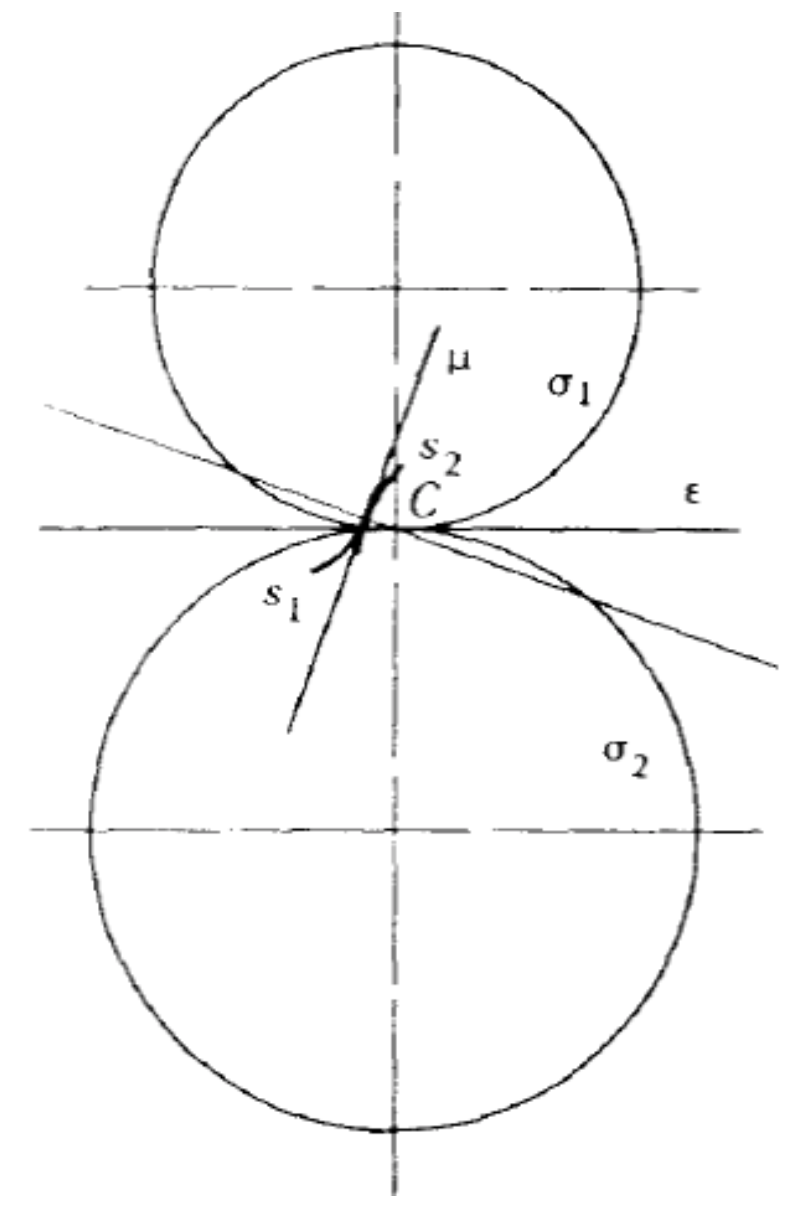
\includegraphics[scale=0.35]{Immagini/EvolventeCilindrica.png}
    \caption{Ruote dentate cilindriche con profilo ad evolvente}
    \label{fig:EvolventeCilindriche}
\end{figure}

Così come per le ruote cilindriche, i profili prevalentemente impiegati nelle ruote coniche sono profili ad evolvente, o meglio, profili prossimi ad evolventi sferici e il dimensionamento è del tutto analogo a quello delle ruote cilindriche. \\
\begin{figure}[h]
    \centering
    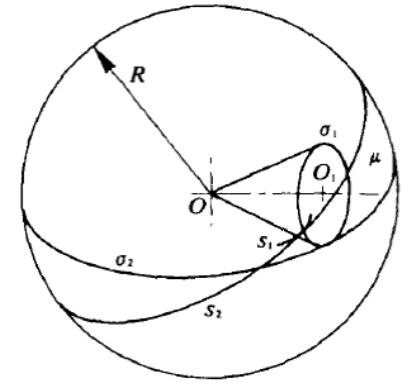
\includegraphics[scale=0.4]{Immagini/EvolventeConica.png}
    \caption{Ruote dentate coniche con profilo ad evolvente}
    \label{fig:EvolventeConica}
\end{figure}
\\
La curva ad evolvente è definita come:
\begin{equation}
    \theta=inv(\alpha)=\tan(\alpha)-\alpha
\end{equation}
\begin{figure}[h]
    \centering
    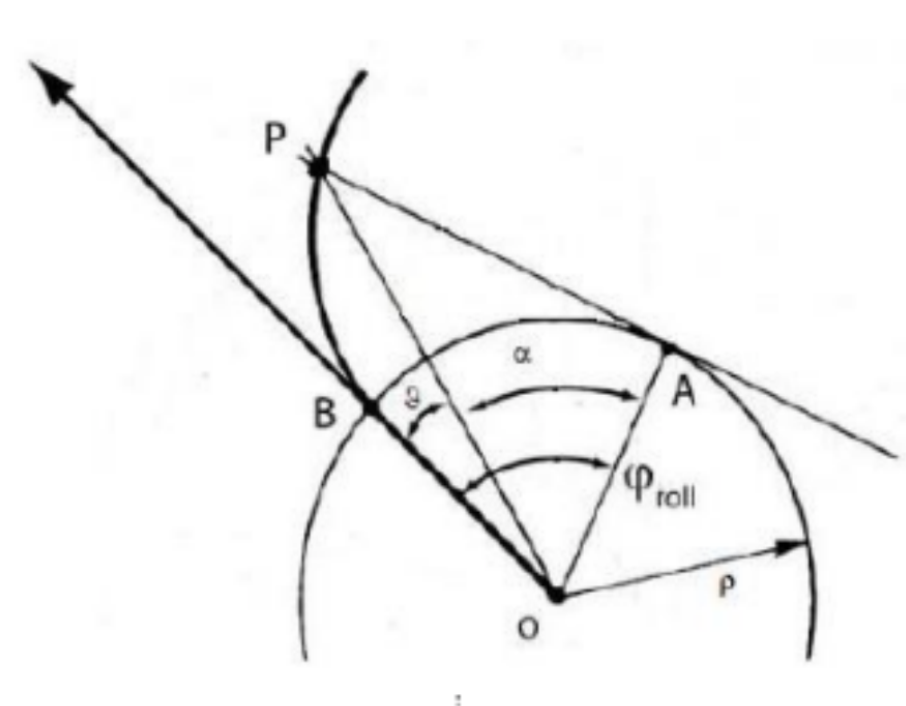
\includegraphics[scale=0.25]{Immagini/Evolvente.png}
    \caption{Generazione del profilo ad evolvente}
    \label{fig:Evolvente}
\end{figure}

Per un generico ingranamento, si identifica con:
\begin{itemize}
    \item $\rho_1$ e $\rho_2$ i raggi di base: raggi delle circonferenze su cui la retta generatrice del fianco del dente rotola senza strisciare, generando il profilo del dente (evolvente di cerchio).
    \item $r_1$ e $r_2$ i raggi primitivi: raggi la cui somma definisci l'interasse, cioè la distanza tra i due centri delle due ruote dentate. 
    \item C centro istantaneo di rotazione: unico punto in cui i due raggi primitivi si toccano e avviene la condizione di puro rotolamento, al di fuori di questo punto si verifica anche la condizione  di strisciamento. 
    \item $\alpha$ angolo di pressione: angolo della linea di azione rispetto all'orizzontale (solitamente $20^{\circ}$).
    \item $a$ interasse. 
\end{itemize}
\begin{figure}[h]
    \centering
    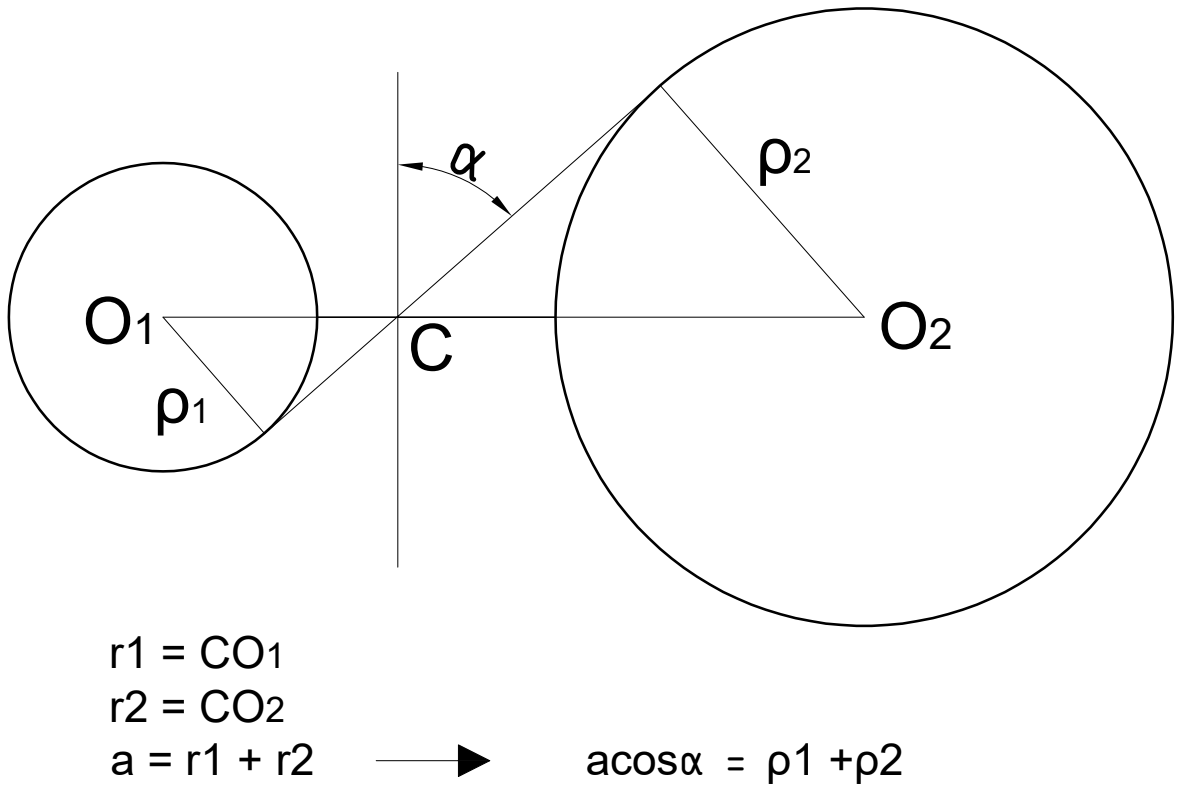
\includegraphics[scale=0.26]{Immagini/Ingranamento.png}
    \caption{Ingranamento tra due ruote dentate}
    \label{fig:Ingranamento}
\end{figure}

Il dimensionamento delle ruote dentate è di tipo modulare: quasi tutti i parametri geometrici della ruota fanno riferimento al modulo m definito come rapporto tra il diametro primitivo d ed il numero di denti Z della ruota, cioè:
\begin{equation}
    m=\frac{d}{Z}.
\end{equation}
Dal modulo (cioè dal numero di denti e dal diametro della primitiva) risulta direttamente determinato il passo (circolare o circonferenziale), che è la distanza tra punti omologhi di due denti consecutivi misurato sulla primitiva:
\begin{equation}
    p=\pi\cdot m=\frac{\pi\cdot d}{Z}.
\end{equation}
Il rapporto di trasmissione può essere espresso mediante la seguente relazione:
\begin{equation}
    \tau=\frac{\omega_1}{\omega_2}=\frac{r_2}{r_1}=\frac{Z_2}{Z_1}.
\end{equation}

\subsection{Geometria del dente}
\begin{figure}[h]
    \centering
    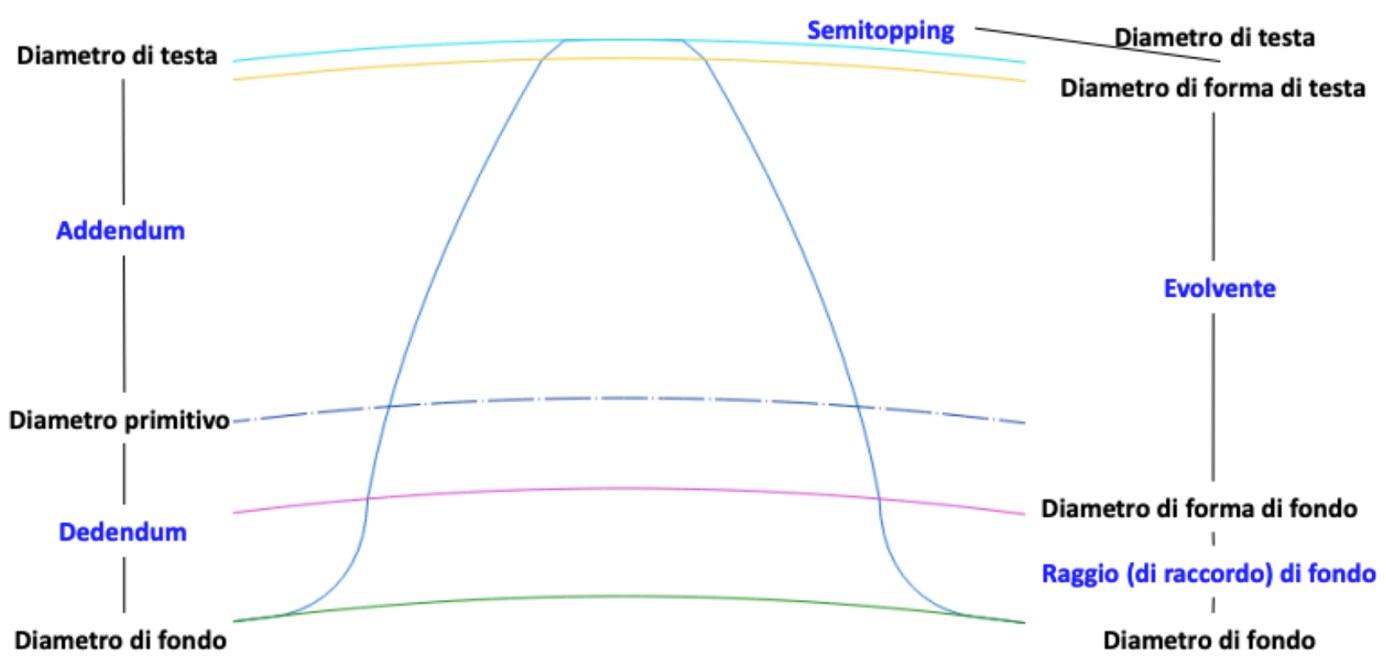
\includegraphics[scale=0.35]{Immagini/FormaDente.png}
    \caption{Forma del dente}
    \label{fig:FormaDente}
\end{figure}

Si definiscono i seguenti parametri descrittivi della forma del dente:
\begin{itemize}
    \item Diametro di testa: diametro della circonferenza che limita superiormente il dente. 
    \item Diametro di piede: diametro della circonferenza che limita inferiormente il dente. 
    \item Diametro primitivo: diametro relativo al luogo dei centri di istantanea rotazione (circonferenza primitiva).
    \item Evolvente: zona di ingranamento tra due denti, che inizia con il diametro di forma di fondo e termina con il diametro di forma di testa. 
    \item Semitopping: smusso realizzato per evitare la rottura dello spigolo del dente durante la sua realizzazione. 
    \item Addendum: estensione in altezza del dente esternamente alla primitiva. 
    \item Dedendum: estensione in altezza del dente internamente alla primitiva.
    \item Fianco: superficie del dente tra primitiva e circonferenza di Dedendum.
    \item Larghezza: spessore del dente nel piano normale alla primitiva. 
\end{itemize}
\newpage
I diametri di fondo siccome delimitano l’evolvente sono propri di una singola ruota dentata. Quando una ruota dentata ingrana con un’altra, si avrà una porzione di evolvente coinvolta nel
contatto e una porzione non coinvolta.\\
La parte di evolvente coinvolta nel contatto è delimitata dai diametri attivi.
\begin{figure}[h]
    \centering
    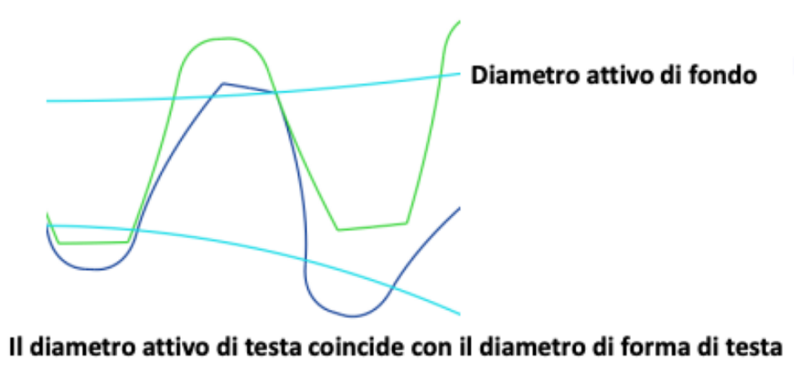
\includegraphics[scale=0.5]{Immagini/DiametriAttivi.png}
    \caption{Diametri attivi}
    \label{fig:DiametriAttivi}
\end{figure}

Questi diametri non sono propri di una ruota, ma dipendono dall’ingranamento. Essi sono quindi propri di una coppia di ruote che ingranano tra loro.\\
Il diametro attivo di testa coincide con quello di forma, perché l’ingranamento arriva fino in punta al dente. Il diametro attivo di fondo deve sempre essere maggiore del diametro di forma di fondo.\\
Bisogna sempre lasciare una porzione che sicuramente non ingranerà perché altrimenti possono verificarsi delle concentrazioni di tensioni.
\subsection{Sollecitazioni}
\begin{figure}[h]
    \centering
    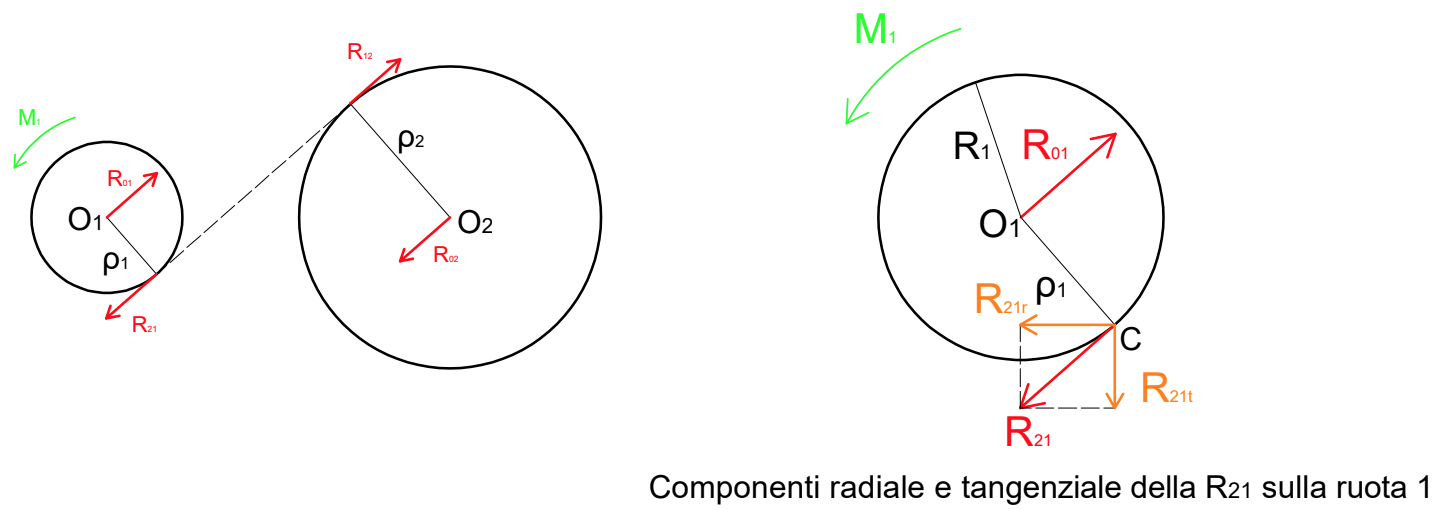
\includegraphics[scale=0.6]{Immagini/ForzeTrasmesse.png}
    \caption{Forze scambiate dalle ruote durante l'ingranamento}
    \label{fig:ForzeTrasmesse}
\end{figure}

Le due ruote ingranando trasmettono un momento, quindi i due denti toccandosi si trasmettono una reazione
uguale e contraria R21 e R12.
Questa reazione ha una componente radiale e una tangenziale.
La componente radiale non da momento, perché passa per il centro della ruota, mentre  la componente tangenziale è quella che trasmette la coppia.
\newpage
\subsubsection{Flessione alla base del dente - Bending}
\begin{figure}[h]
    \centering
    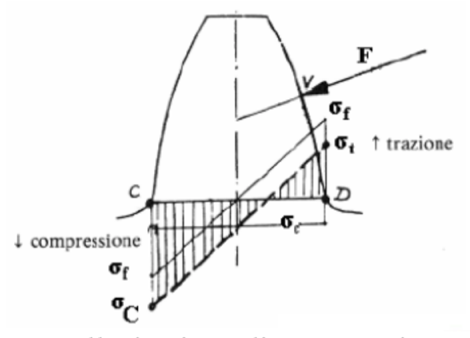
\includegraphics[scale=0.7]{Immagini/Bending1.png}
    \caption{Andamento delle sollecitazioni dovute a Bending}
    \label{fig:Bending1}
\end{figure}

La componente radiale genera una sollecitazione di compressione sul dente, mentre quella tangenziale genera una sollecitazione di flessione con un andamento di tipo farfalla simmetrica, quindi sommando i due contributi il risultato ottenuto è un andamento a farfalla asimmetrica. Il raccordo alla base del dente è l'elemento maggiormente sottoposto a questo tipo di sollecitazione (punto D 
sollecitato a trazione e C a compressione).\\
La sollecitazione a cui è sottoposto un dente non è statica, ma è affaticante all’origine, poichè durante l'ingranamento questi ultimi vengono caricati in punti diversi del loro fianco, fino a scaricarsi completamente per ogni ciclo.\\
\\
Con il metodo FEM è possibile stimare la distribuzione delle sollecitazioni sul fondo del dente, dove il colore blu rappresenta una sollecitazione ridotta mentre il colore rosso una sollecitazione rilevante. 
\begin{figure}[h]
    \centering
    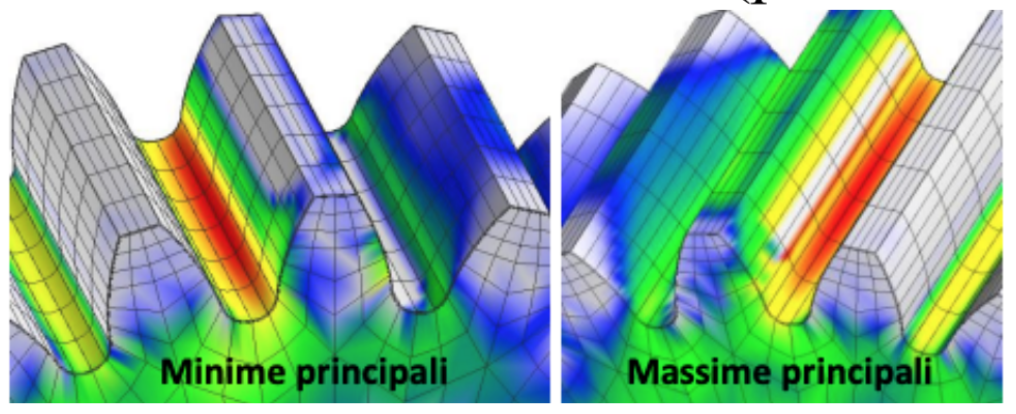
\includegraphics[scale=0.4]{Immagini/FEM.png}
    \caption{Analisi FEM delle sollectazioni a flessione}
    \label{fig:FEM}
\end{figure}
\subsubsection{Pressioni di contatto sul fianco del dente - Pitting}
\begin{figure}[h]
    \centering
    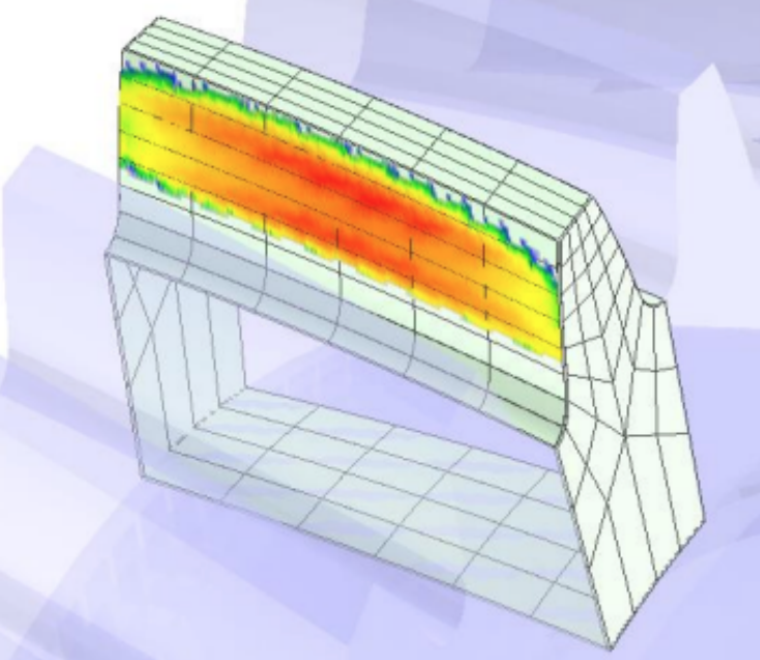
\includegraphics[scale=0.3]{Immagini/Pitting.png}
    \caption{Sollecitazione di compressione}
    \label{fig:Pitting}
\end{figure}
Le ruote ingranando trasmettono la coppia attraverso la compressione dei denti, questa sollecitazione genera delle pressioni di contatto che agiscono sul fianco del dente.\\
\\
Il contatto tra i due denti è un contatto definito non conforme. Idealmente le due superfici concave  si trasmettono pressioni di contatto attraverso un punto alla volta lungo la sezione, mentre attraverso una linea lungo la fascia del dente. In realtà il contatto avviene in una porzione a forma di ellisse
che durante l’ingranamento si sposta lungo il profilo, dal fondo alla testa del dente.\\
Queste pressioni di contatto aumentano all’aumentare del carico, più carico l'ingranaggio deve trasmettere, più le pressioni sono elevate.\\
Queste sollecitazioni seguono la teoria di Hertz: comprimendo si genera una pressione che causa delle sollecitazioni, che variano dalla superficie alla sotto-superficie e che trovano un massimo in uno strato sotto-superficiale.\\
Le pressioni di contatto, come dice il nome, sono presenti solamente quando il dente è in presa, quindi la compressione avrà un andamento di tipo ciclo affaticante. 
\subsubsection{Strisciamento}
Durante il contatto tra i denti delle due ruote, l'ingranamento varia a seconda della posizione del contatto. Infatti, il centro istantaneo di rotazione vedrà una condizione di puro rotolamento, al contrario di qualsiasi altro punto che subirà rotolamento e strisciamento.\\
Quest'ultimo fenomeno risulta particolarmente dannoso in quanto determina asportazione di materiale, risulta quindi di particolare interesse limitarne il più possibile gli effetti. \\
\\
L'andamento dell'entità dello strisciamento è rappresentata in Fig.\ref{fig:Strisciamento}.
\begin{figure}[h]
    \centering
    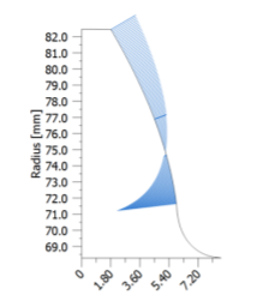
\includegraphics[scale=0.65]{Immagini/Strisciamento.png}
    \caption{Andamento dello strisciamento lungo il fianco del dente}
    \label{fig:Strisciamento}
\end{figure}
\\
Si noti come, allontanandosi dal centro istantaneo di rotazione C (in corrispondenza del diametro primitivo), l'entità dello strisciamento aumenta, risultando massima in testa e alla base del dente.\\
Calcolare però l’effetto dello strisciamento risulta essere complicato perché non entra in gioco solo la resistenza del materiale, ma anche altri fattori come ad esempio la lubrificazione. Infatti, le superfici dei denti non sono a contatto diretto, ma vi si interpone un meato di lubrificante (olio) per prevenire appunto l’usura da strisciamento.
\subsection{Failure modes}
Durante la progettazione risulta necessario tenere conto di tutte le sollecitazioni sopra elencate, altrimenti si può incorrere in danneggiamenti di diverso tipo.\\
Si illustrano dunque alcune modalità di guasto che si possono presentare relativamente ad un ingranaggio.
\subsubsection{Bending}
Rottura alla base del dente dovuta a flessione affaticante, che presenta il suo massimo in corrispondenza del raccordo alla base dello stesso.
\begin{figure}[h]
    \centering
    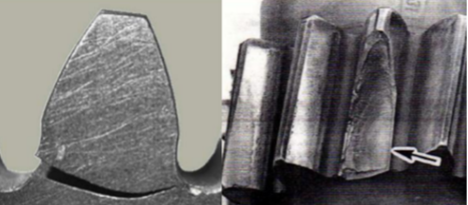
\includegraphics[scale=0.7]{Immagini/Bending2.png}
    \caption{Rottura a Bending del dente}
    \label{fig:Bending2}
\end{figure}
\subsubsection{Pitting}
Creazione di crateri (pits) sulla superficie del dente a causa della fatica da contatto. 
Si formano inizialmente dove la pressione di contatto è più elevata (generalmente nell’intorno del diametro primitivo), per poi estendersi su tutta la superficie del dente.\\ 
Per la teoria di Hertz si presenta un picco di tensione nella sotto-superficie. In quel punto si genera una cricca che poi raggiunge la superficie facendo staccare una porzione di materiale nell’intorno della cricca (cratere). I vari crateri si congiungono l’uno all’altro fino a “mangiare” completamente tutto il dente. 
Il dente arriva ad assottigliarsi talmente tanto da staccarsi durante l’ingranamento.
\begin{figure}[h]
    \centering
    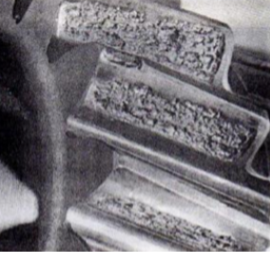
\includegraphics[scale=0.7]{Immagini/Pitting2.png}
    \caption{Rottura a Pitting del dente}
    \label{fig:Pitting2}
\end{figure}
\subsubsection{Micropitting}
Fenomeno per il quale si formano dei micro-crateri generati dal contatto tra le microasperità della superficie locale di metallo contro metallo. È una modalità di guasto dovuta a un film di lubrificante troppo sottile. \\
Se non si interpone una quantità sufficiente di lubrificante, le microasperità si saldano tra loro e durante lo strisciamento vengono asportate.\\
Il Micropitting può rimanere stabile durante il funzionamento oppure degenerare in vero e proprio Pitting. 
\begin{figure}[h]
    \centering
    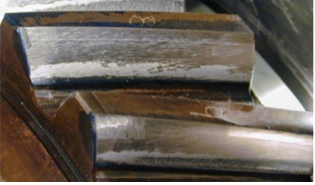
\includegraphics[scale=0.7]{Immagini/Micropitting.png}
    \caption{Rottura a Micropitting del dente}
    \label{fig:Micropitting}
\end{figure}
\subsubsection{Scuffing}
Fenomeno per il quale si generano alcuni segni verticali causati dall’effetto combinato di elevate velocità di strisciamento e pressioni di contatto, che causano la rottura del film lubrificante e il conseguente contatto metallo contro metallo e le problematiche prima descritte (come le microsaldature).
\begin{figure}[h]
    \centering
    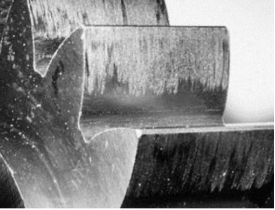
\includegraphics[scale=0.7]{Immagini/Scuffing.png}
    \caption{Rottura del dente a Scuffing}
    \label{fig:Scuffing}
\end{figure}
\section{Progettazione}
In primo luogo è stato eseguito un dimensionamento di massima degli ingranaggi, svolgendo i vari calcoli per il dimensionamento delle diverse ruote del riduttore. In seguito, è stato utilizzato il software di calcolo KissSoft per effettuare il dimensionamento vero e proprio. \\
Il riduttore è dotato di un solo ingresso (input) e di due uscite coassiali (output 1 e output 2), analizzate separatamente. 
\subsection{Dati di progetto}
Per la progettazione sono state considerate le seguenti velocità:
\begin{itemize}
    \item INPUT: velocità di rotazione dell'albero pari a 312 rpm;
    \item OUTPUT 1: velocità di rotazione dell'albero pari a 23 rpm;
    \item OUTPUT 2: velocità di rotazione dell'albero pari a 719 rpm.
\end{itemize}
\newpage
Il carico considerato è riportato in Fig.\ref{fig:Carico}.
\begin{figure}[h]
    \centering
    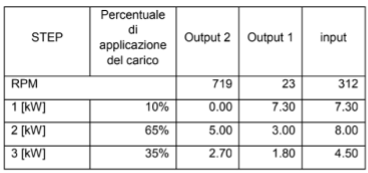
\includegraphics[scale=0.9]{Immagini/Carico.png}
    \caption{Ciclo di carico a cui è sottoposto il riduttore}
    \label{fig:Carico}
\end{figure}
\\
L’angolo di inclinazione d’elica è stato supposto pari a $\beta=20^\circ$. \\
Inoltre, a seguito di numerosi tentativi è stato supposto un interasse I pari a 170 mm.\\
\\
I materiali scelti per la realizzazione degli ingranaggi sono acciai da cementazione e, in questo caso, si è scelto 20MnCr5.\\
\\
Qualità richiesta dagli ingranaggi:
\begin{itemize}
    \item Ingranaggi conici: DIN3965 Qualità 9;
    \item Ingranaggi cilindrici ISO1328 Qualità 9.
\end{itemize}
Per la realizzazione degli alberi è stato utilizzato il materiae 42CrMo4.\\
\\
La durata richiesta per il riduttore è pari a 3600h, sarà necessario quindi prevedere opportuni coefficienti di sicurezza secondo ISO6336 e ISO10300: 
\begin{itemize}
    \item SF Bending $>$ 1.3;
    \item SF Pitting $<$ 1.1 .
\end{itemize}
Il lubrificante utilizzato è il \textit{SPIRAX S3 AX 80W-90}, dotato delle seguenti caratteristiche:
\begin{figure}[h]
    \centering
    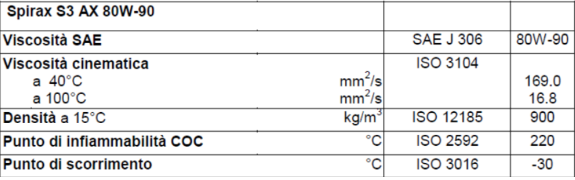
\includegraphics[scale=0.9]{Immagini/Lubrificante.png}
    \caption{Caratteristiche del lubrificante impiegato}
    \label{fig:Lubrificante}
\end{figure}
\subsection{Dimensionamento preliminare}
Con i dati forniti dall’azienda Comer è stato possibile calcolare il rapporto di trasmissione totale prima della trasmissione input – output 1 e poi di quella input – output 2 come: 
\begin{equation}
    \tau_{tot1}=\frac{n_{21}}{n_1}=0.074
\end{equation}
\begin{equation}
        \tau_{tot2}=\frac{n_{22}}{n_1}=2.30
\end{equation}
Ricordando poi che $\tau_{tot1}=\tau_{01}\cdot\tau_{23}\cdot\tau_{45}$ e che $\tau_{tot2}=\tau_{01}\cdot\tau_{23}\cdot\tau_{67}$, sono stati supposti i singoli rapporti di trasmissione rispettando le equazioni appena scritte. \\
L'approccio seguito ha visto diverse iterazioni dei vari rapporti fino a trovare una configurazione idonea sia in termini di ingombri che di rapporto di riduzione totale.\\
Sono stati assunti i singoli rapporti di trasmissione pari a: 
\begin{itemize}
    \item $\tau_{01}=0.84$;
    \item $\tau_{23}=0.45$;
    \item $\tau_{45}=0.19$;
    \item $\tau_{67}=6$.
\end{itemize}
Il rapporto di trasmissione si definisce anche come rapporto tra il numero di denti tra i due ingranaggi:
\begin{equation}
    \tau=\frac{z_2}{z_1}.
\end{equation}
Supposto quindi il rapporto di trasmissione di ogni coppia di ingranaggi, è stata costruita su Excel una tabella che riportasse le diverse combinazioni di numeri di denti che portavano allo stesso valore di rapporto di trasmissione. 
\begin{figure}[h]
    \centering
    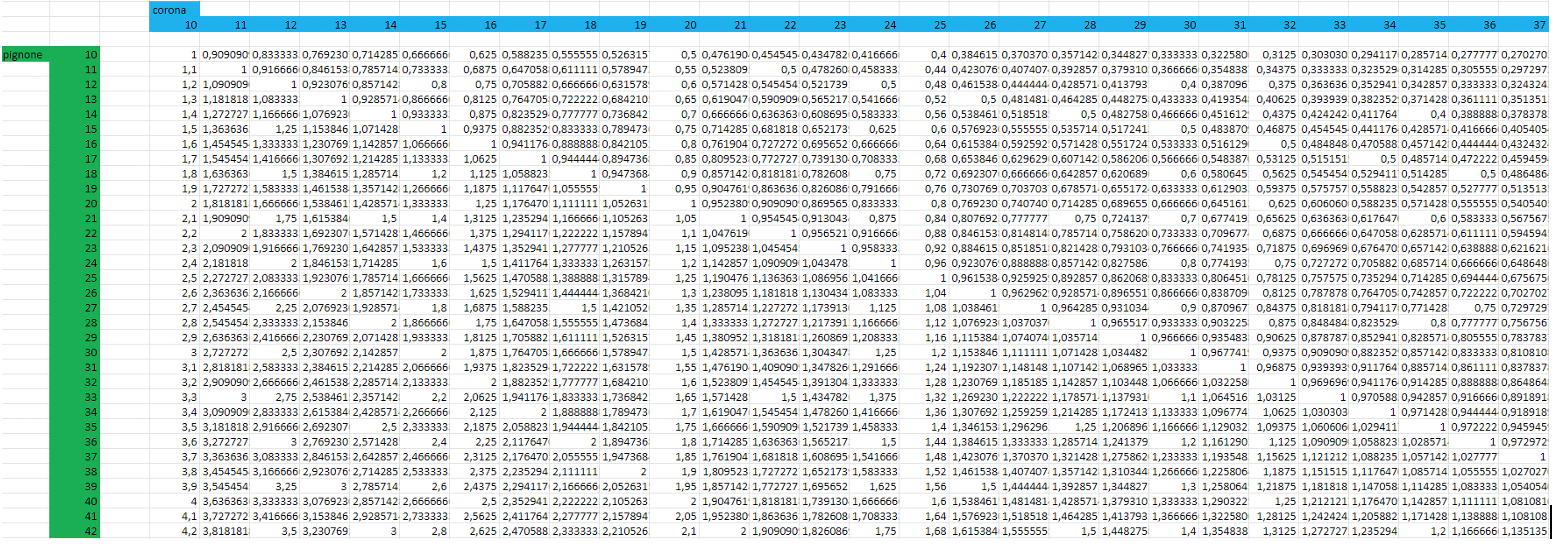
\includegraphics[scale=0.5]{Immagini/Excel.png}
    \caption{Combinazioni dei numeri di denti che fornisce lo stesso rapporto di trasmissione}
    \label{fig:Excel}
\end{figure}
\\
In questo modo sono state trovate diverse combinazioni di numeri di denti di corona e pignone di ogni singolo ingranaggio.\\
I numeri di denti trovati sono stati poi il punto di partenza per la progettazione mediante software KissSoft. 
\subsection{Dimensionamento tramite software KissSoft}
Il dimensionamento tramite software KissSoft è stato fatto singolarmente per ogni coppia di ruote dentate: 
\begin{itemize}
    \item Coppia 0 1;
    \item Coppia 2 3;
    \item Coppia 4 5;
    \item Coppia 6 7;
\end{itemize}
Le prime due coppie di ruote 0 1 e 2 3 sono coppie coniche, mentre le coppie 4 5 e 6 7 sono coppie cilindriche. 
\subsubsection{Dimensionamento coppie cilindriche}
\paragraph{Metodologia applicata per il dimensionamento}
In primo luogo, sono stati verificati gli ingombri di massima di ogni coppia di ruote, a partire dai dati di progetto forniti.\\
Una volta aperto il KissSoft per la prima coppia di ruote cilindriche, sono stati inseriti i “dati base” ottenuti dal dimensionamento di preliminare, cioè le diverse combinazioni di numeri di denti delle coppie di ruote e un certo valore supposto del modulo. Andando poi a supporre la larghezza del dente, è stato calcolato dal software il valore dell’interasse e successivamente è stato verificato che esso rientrasse nei limiti geometrici imposti. \\
Agendo per tentativi, variando il modulo o il numero di denti (sempre rispettando il rapporto di trasmissione supposto), si è cercato di far avvicinare il più possibile l’interasse al valore più adatto a rispettare gli ingombri imposti. Una volta raggiunto un valore di interasse vicino a quello ottimale, cioè 170 mm, si è ottenuta di conseguenza la relativa configurazione geometrica della coppia di ruote.\\
\\
Il procedimento è stato ripetuto analogamente per ogni coppia di ruote dentate.\\
\\
Si è cercato di evitare un valore negativo del fattore di spostamento del profilo x, quindi la logica di dimensionamento seguita ha portato al migliore compromesso tra modulo, numero di denti, interasse conseguente e fattore di spostamento non negativo. \\
Il software calcola in automatico diversi valori di correzione in base a vari parametri. Tra le varie opzioni disponibili si è scelto “Per scorrimento specifico ottimale”, in modo da distribuire l’usura dovuta allo strisciamento analogamente su entrambi i denti così da minimizzare il pitting.
\begin{figure}[h]
    \centering
    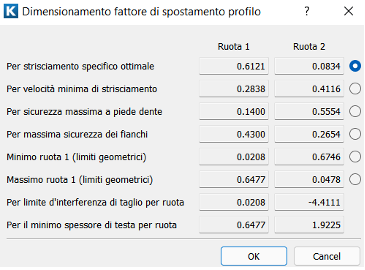
\includegraphics{Immagini/MetodologiaDimensionamentoCilindriche.png}
    \caption{Dimensionamento fattore di spostamento del profilo}
    \label{fig:MetodologiaDimensionamentoCilindriche}
\end{figure}
\paragraph{Progettazione macrogeometrica ingranaggi cilindrici}
In seguito al calcolo dei fattori di sicurezza ci si è trovati in situazioni in cui la resistenza a Bending poteva essere sovradimensionata rispetto al Pitting (e viceversa), oppure che uno dei due fattori (o entrambi) non raggiungesse il valore minimo accettabile.\\
Per risolvere questa problematica si è agito su diversi elementi del dimensionamento:
\begin{itemize}
    \item Incremento di larghezza del dente b. Questa soluzione determina un miglioramento sia a Bending che a Pitting, pertinente quindi nel caso in cui entrambi i coefficienti risultano sottodimensionati. 
    \item Decremento del modulo, corrispondente ad un aumento del numero di denti (a parità di interasse). Soluzione che penalizza la resistenza a Bending in favore della resistenza a Pitting. 
    \item Massimizzazione del raggio di raccordo al piede del dente, in direzione di un incremento del fattore di sicurezza a Bending. 
    \item Incremento dell'altezza del dente, il quale si traduce in un incremento dell'addendum del creatore. Scavando di più il dente si migliora la resistenza a Pitting. 
\end{itemize}
Risulta buona norma di progettazione considerare un fattore di ricoprimento maggiore o uguale ad 1 (ancora meglio se superiore ad 1.3-1.4). Questo perché il ricoprimento è indicativo della superficie di contatto e tanto più sarà maggiore, tanto minori saranno le tensioni relative alle pressioni contatto.\\
Questo risultato è ottenibile ad esempio alzando l'altezza dei denti di entrambe le ruote, comportando però maggiore sollecitazione flessionale (Bending). 
\paragraph{Progettazione microgeometrica ingranaggi cilindrici} La progettazione sin qui svolta da normativa non considera alcuni fattori di cui si deve necessariamente tenere conto. Ad esempio, è possibile andare a calcolare il fattore sulla lunghezza del dente $K_{HB}$ derivante da un'analisi delle pressioni che agiscono sul dente (pressione massima su pressione media).\\
Se $K_{HB}$ avesse valore unitario, significherebbe che la pressione massima sarebbe uniformemente distribuita lungo tutta la superficie del dente. Si è scelto in via cautelativa di supporre tale fattore leggermente superiore all'unità, per poi verificarlo a posteriori andando a verificare due aspetti:
\begin{itemize}
    \item Micro-modifiche del profilo, sagomando ad hoc il creatore o attraverso rettifica;
    \item Influenza della non infinita rigiità degli alberi.
\end{itemize}

Per modifiche micro-geometriche si intendono modifiche che prevedono l’asportazione di materiale in testa e al piede del dente (scostamento dall’evolvente teorico) per compensare le deformazioni del dente ed evitare quindi gli urti. L’asportazione micro-geometrica di materiale in testa viene chiamata “tip relief”, mentre quella al piede “root relief”. \\
\\
In funzione della loro forma si definiscono:
\begin{itemize}
    \item Lunghe o corte a seconda del diametro dove hanno inizio lungo il profilo (secondo ISO 21771);
    \item Lineari o paraboliche a seconda che siano tratti di retta o parabola sul K-Chart. Solitamente le paraboliche sono preferibili poiché la parabola crea continuità, evitando spigoli che possono determinare fattori di concentrazione delle tensioni. 
\end{itemize}
\newpage
Per effettuare le modifiche è necessario andare nella sezione “Modifiche” del KissSoft e inserire un elenco di nuove asportazioni di materiale.
\begin{figure}[h]
    \centering
    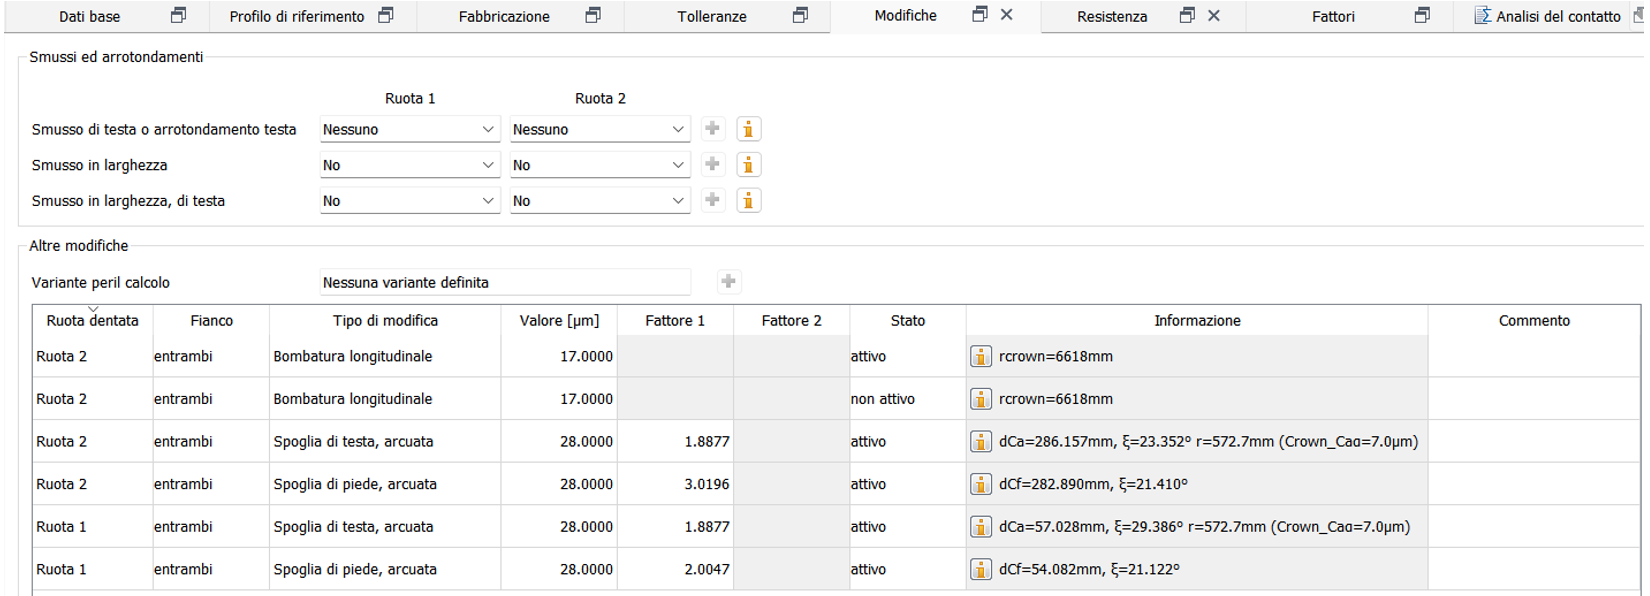
\includegraphics[scale=0.5]{Immagini/ModificheKissSoft.png}
    \caption{Parametri di modifica del software KissSoft}
    \label{fig:ModificheKissSoft}
\end{figure}

È possibile inserire la bombatura longitudinale, la spoglia di testa o di piede, correzione angolo d’elica e tante altre a seconda della necessità.\\
Il fattore 1 indica da dove si vuole far partire la modifica attraverso il tasto di "modifica di massima", dove è possibile andare a decidere quale lavorazione fare, dove e come. 
\begin{figure}[h]
    \centering
    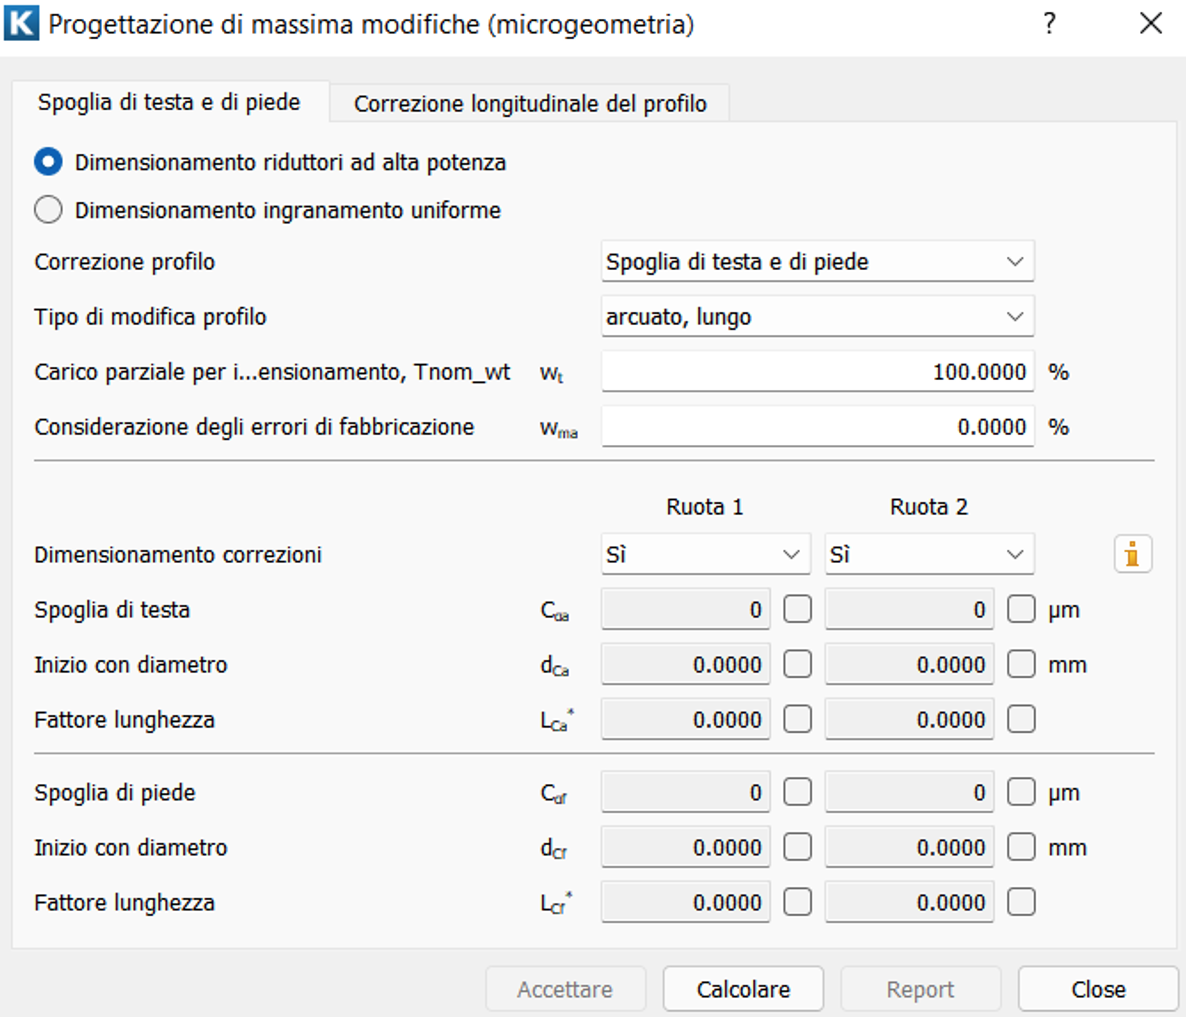
\includegraphics[scale=0.35]{Immagini/ModificheMicrogeometria.png}
    \caption{Modifiche della microgeometria del dente}
    \label{fig:ModificheMicrogeometria}
\end{figure}

Per verificare invece quanto è rigido l’albero è necessario prima progettare l’albero, inserirlo nel KissSoft e vedere come la sua rigidezza, oltre a quella dei denti, influisce sul contatto. In questo modo si riesce anche a verificare a posteriori il $K_{HB}$.
\newpage
\paragraph{Coppia cilindrica 4 5} Definizione dei dati di base della coppia cilindrica.  
\begin{figure}[h]
    \centering
    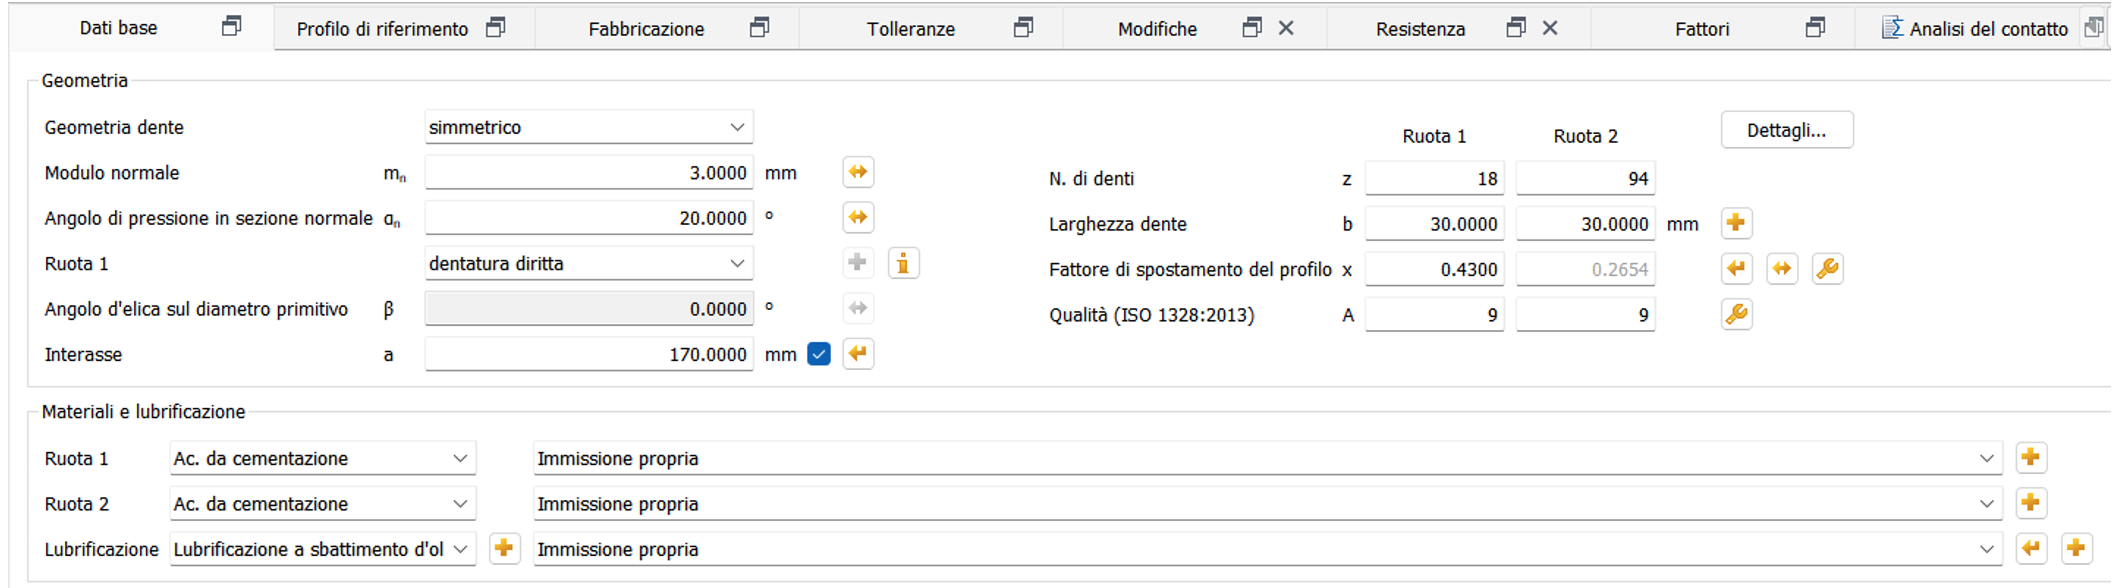
\includegraphics[scale=0.4]{Immagini/Coppia45.png}
    \caption{Dati di base coppia 4 5}
    \label{fig:Coppia45}
\end{figure}

A seguito di diversi tentativi quindi per la prima coppia cilindrica è stato scelto un numero di denti pari a 18 per la ruota 1 e pari a 94 per la ruota 2. Il modulo è stato supposto pari a 3 mm, la larghezza del dente pari a 30 mm, l’angolo di pressione 20° e un interasse pari a 170 mm, ideale per rispettare gli ingombri disponibili. La qualità degli ingranaggi pari a 9 (ISO1328). Il materiale scelto per entrambe le ruote è un acciaio da cementazione 20MnCr5, con un carico di rottura $R_m$ pari a $1200\ N/mm^2$ e un carico di snervamento $R_s$ pari a 850 $N/mm^2$. 
\begin{figure}[h]
    \centering
    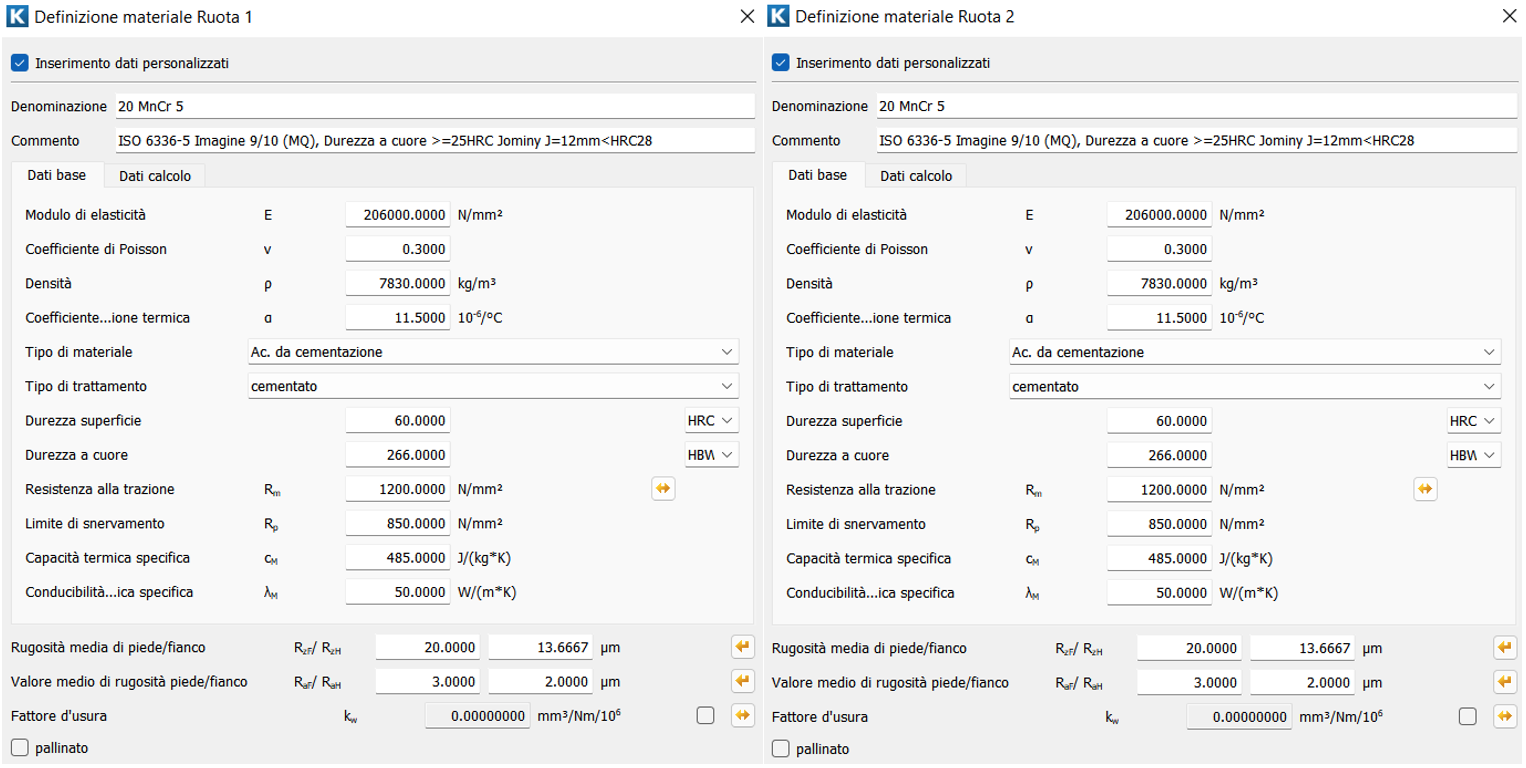
\includegraphics[scale=0.5]{Immagini/RuoteCoppia45.png}
    \caption{Parametri delle ruote della coppia 4 5}
    \label{fig:RuoteCoppia45}
\end{figure}
\newpage
Per quanto riguarda il lubrificante invece non essendo presente tra le scelte del software è stato necessario crearlo procedendo come in Fig.\ref{fig:LubrificanteCoppia45}, inserendo tutti i dati di progetto richiesti. Il lubrificante utilizzato è lo \textit{SPIRAX S3 AX 80W-90}, con le seguenti caratteristiche: 
\begin{figure}[h]
    \centering
    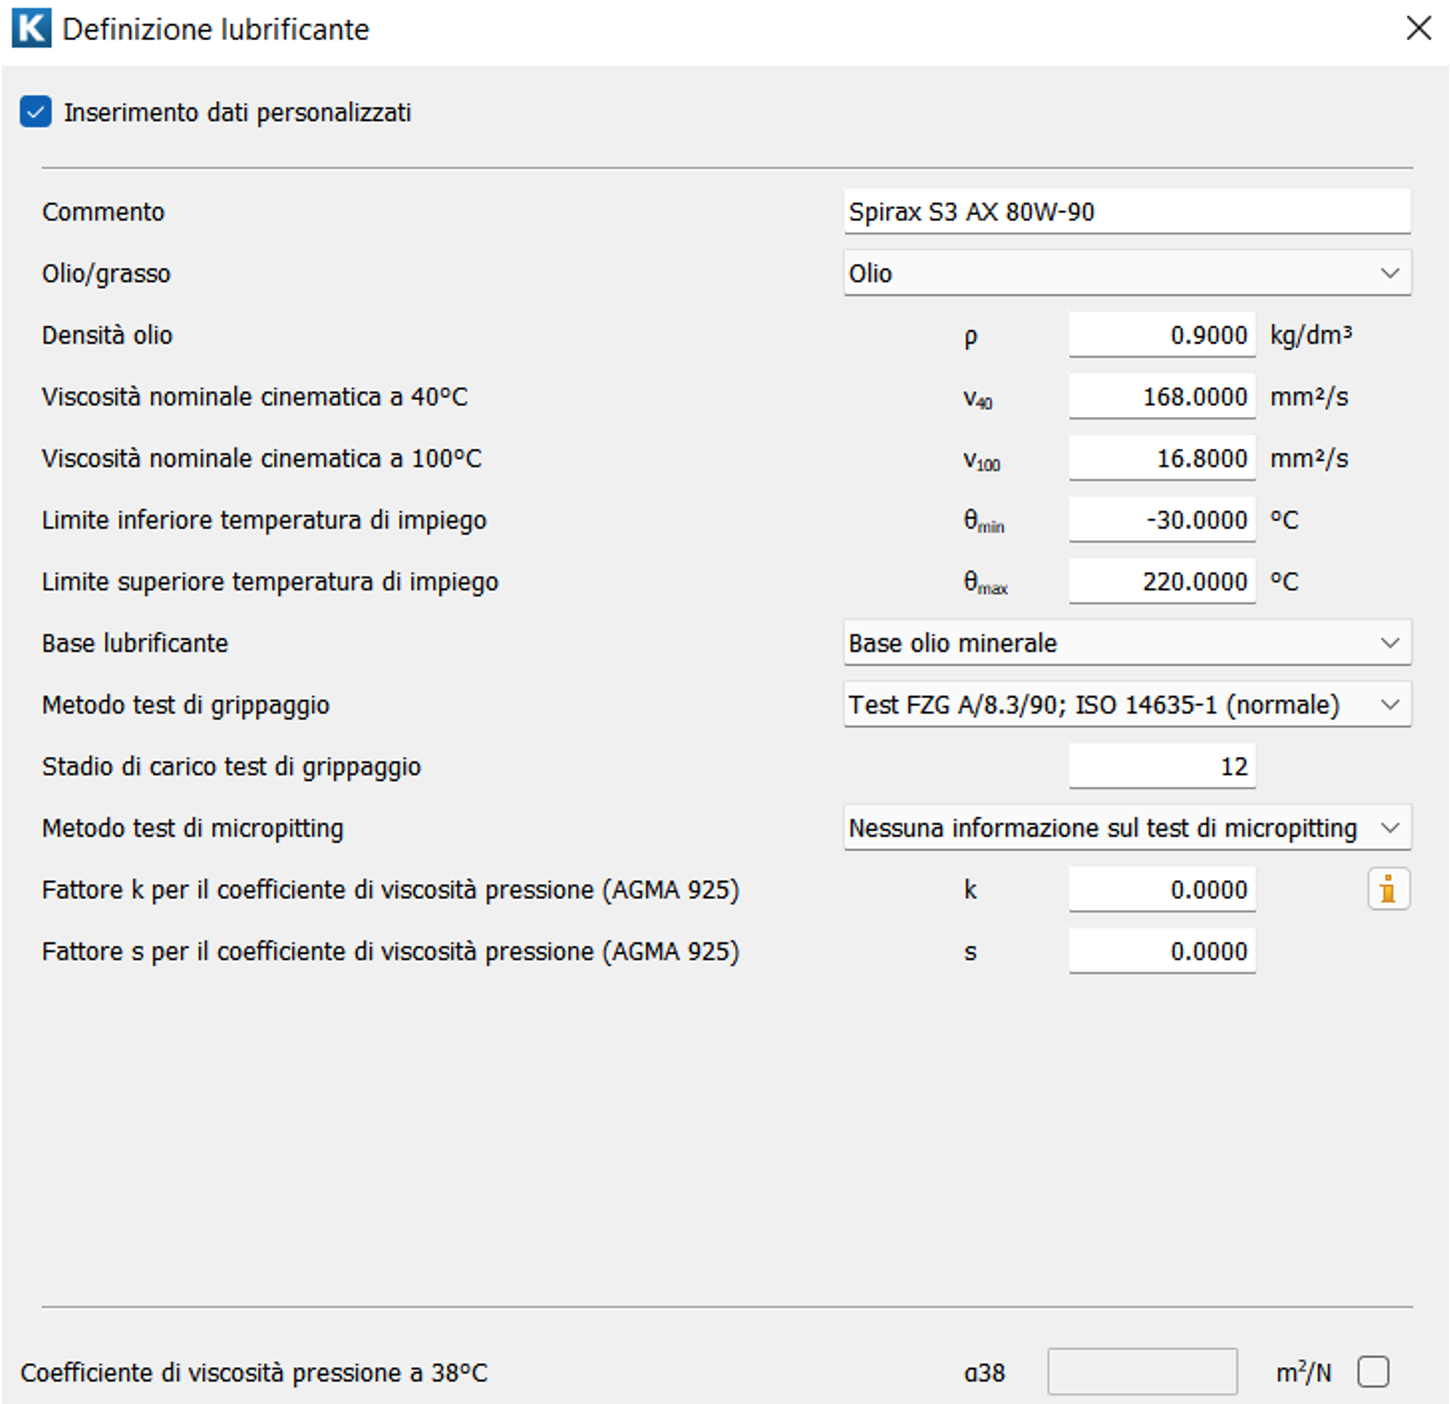
\includegraphics[scale=0.35]{Immagini/LubrificanteCoppia45.png}
    \caption{Parametri caratteristici del lubrificante}
    \label{fig:LubrificanteCoppia45}
\end{figure}

Le altre sezioni del KissSoft per la prima coppia cilindrica sono state così compilate.\\
\\
Sezione \emph{Profilo di riferimento}
\begin{figure}[h]
    \centering
    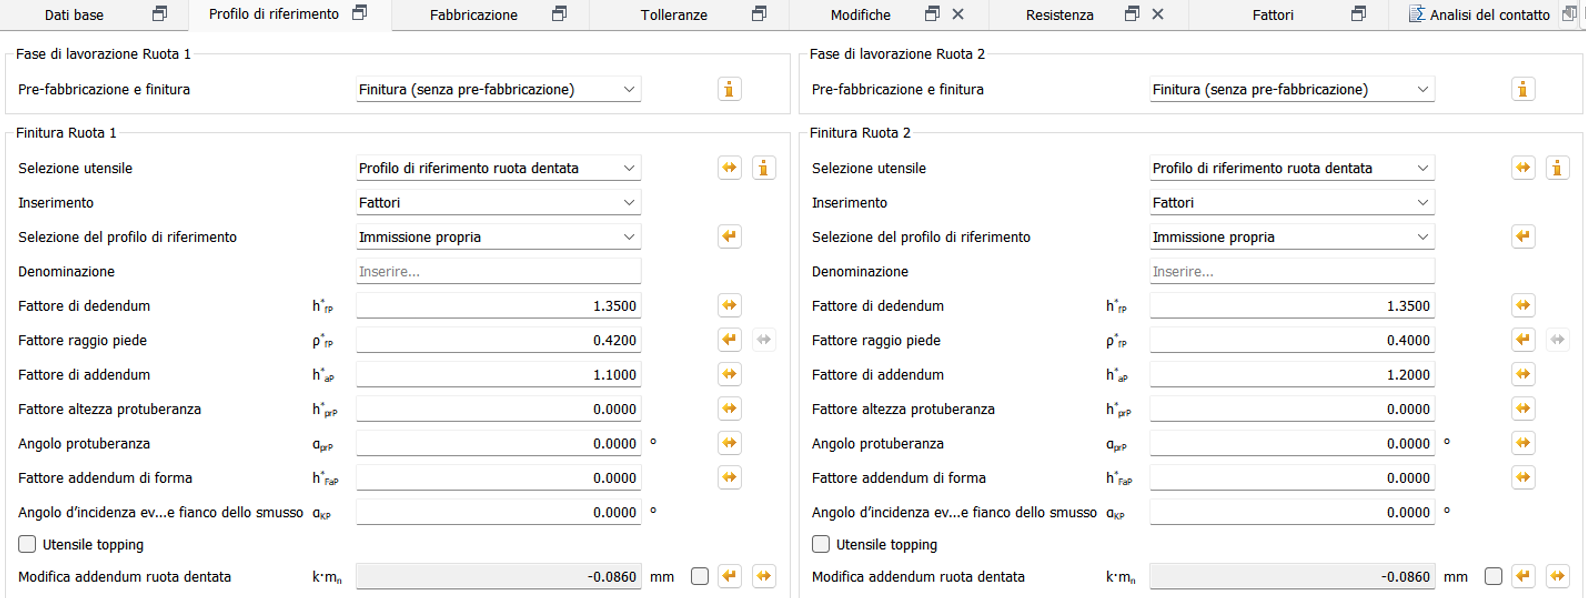
\includegraphics[scale=0.5]{Immagini/ProfiloRiferimentoCoppia45.png}
    \caption{Profilo di riferimento delle due ruote della coppia 4 5}
    \label{fig:ProfiloRiferimentoCoppia45}
\end{figure}

Questa sezione riguarda il tipo di profilo utensile utilizzato per l’inviluppo del dente. 
In generale per ruote standard si utilizza o prefabbricazione o finitura (senza prefabbricazione), come nel caso in esame. Una volta scelto il profilo di riferimento i dati vengo inseriti in automatico dal Software.\\
\newpage
Sezione \emph{Fabbricazione}
\begin{figure}[h]
    \centering
    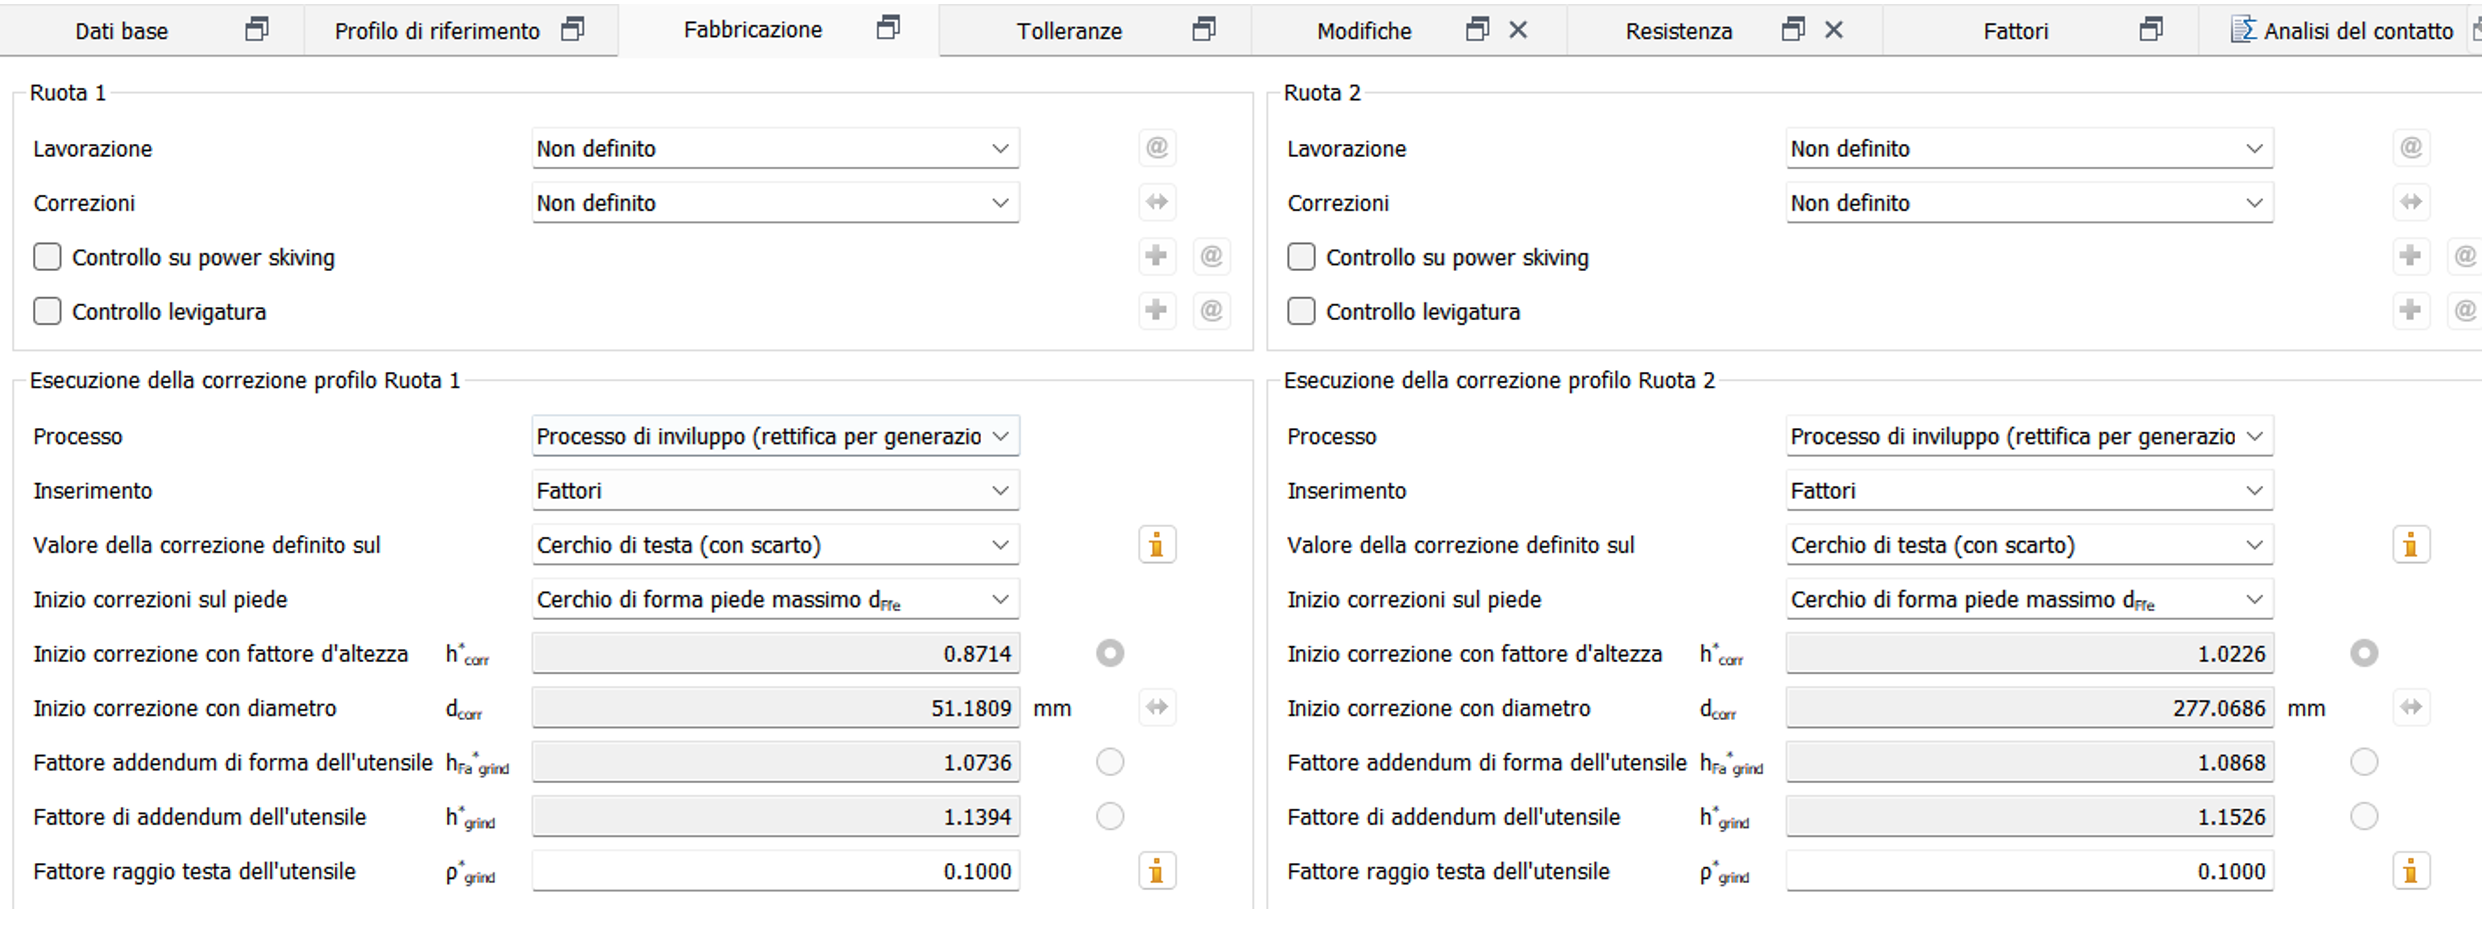
\includegraphics[scale=0.35]{Immagini/FabbricazioneCoppia45.png}
    \caption{Parametri di fabbricazione delle ruote della coppia 4 5 }
    \label{fig:FabbricazioneCoppia45}
\end{figure}

Sezione \emph{Tolleranze}
\begin{figure}[h]
    \centering
    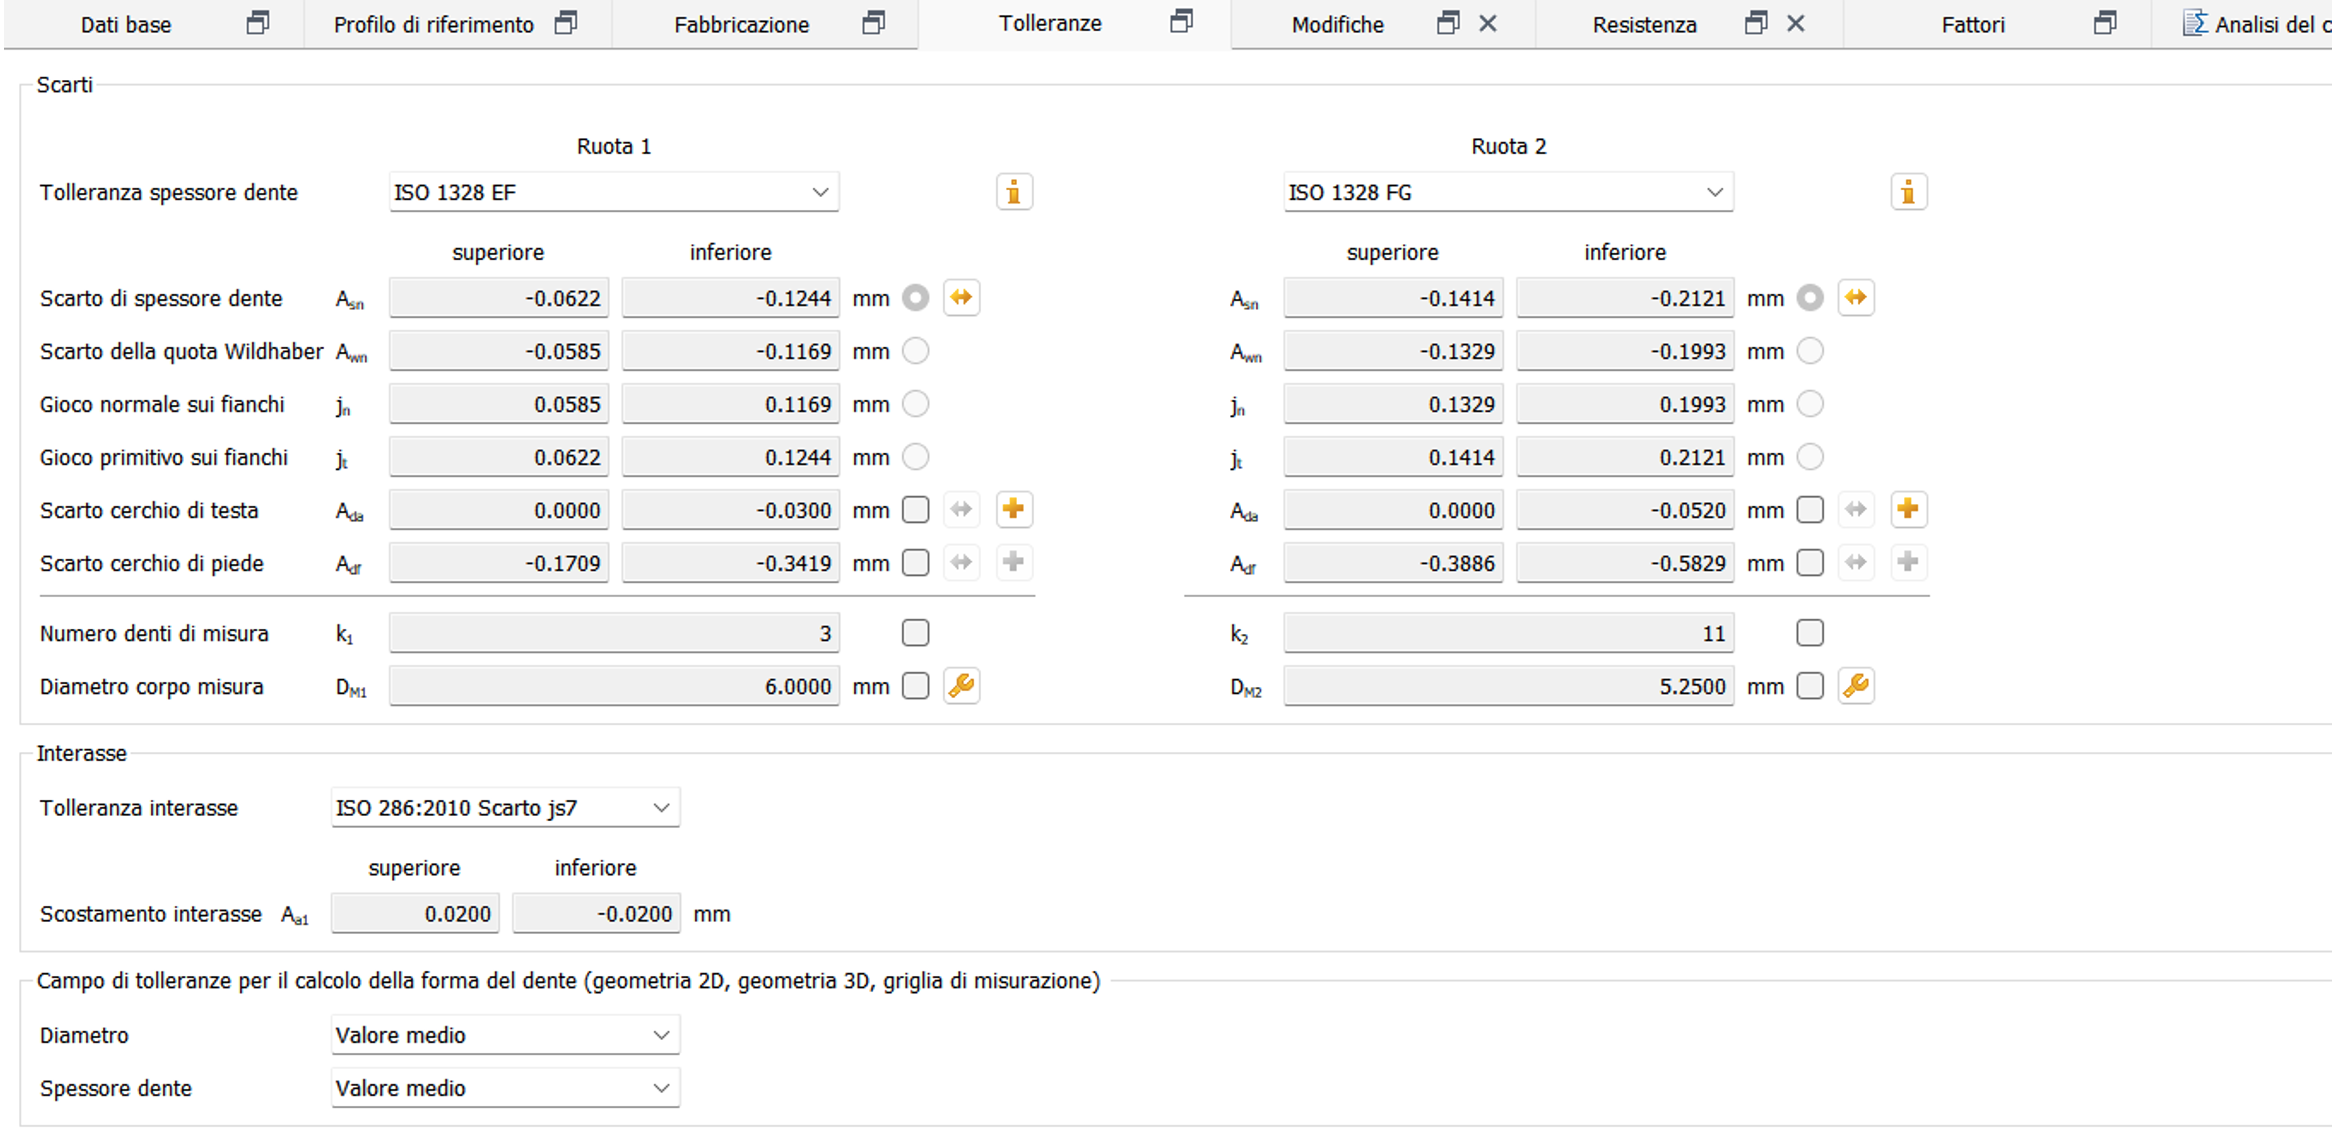
\includegraphics[scale=0.4]{Immagini/TolleranzeCoppia45.png}
    \caption{Tolleranze delle ruote della coppia 4 5}
    \label{fig:TolleranzeCoppia45}
\end{figure}

Questa sezione permette di inserire le diverse tolleranze relative agli scarti e interasse, all’interno di “Scarti” compare la voce “Tolleranza spessore dente”, dove è stata scelta la tipologia di tolleranza in base alla normativa ISO1328. Per quanto riguarda la tolleranza all’interasse è stata scelta la voce ISO 286:2010 Scarto js7.\\
Le tolleranze non sono importanti per la parte di calcolo dell’ingranaggio, ma sono funzionali al disegno. La tolleranza più importante è quella della testa del dente, funzionale per la fase di tornitura. 
\newpage
Sezione \emph{Modifiche}
\begin{figure}[h]
    \centering
    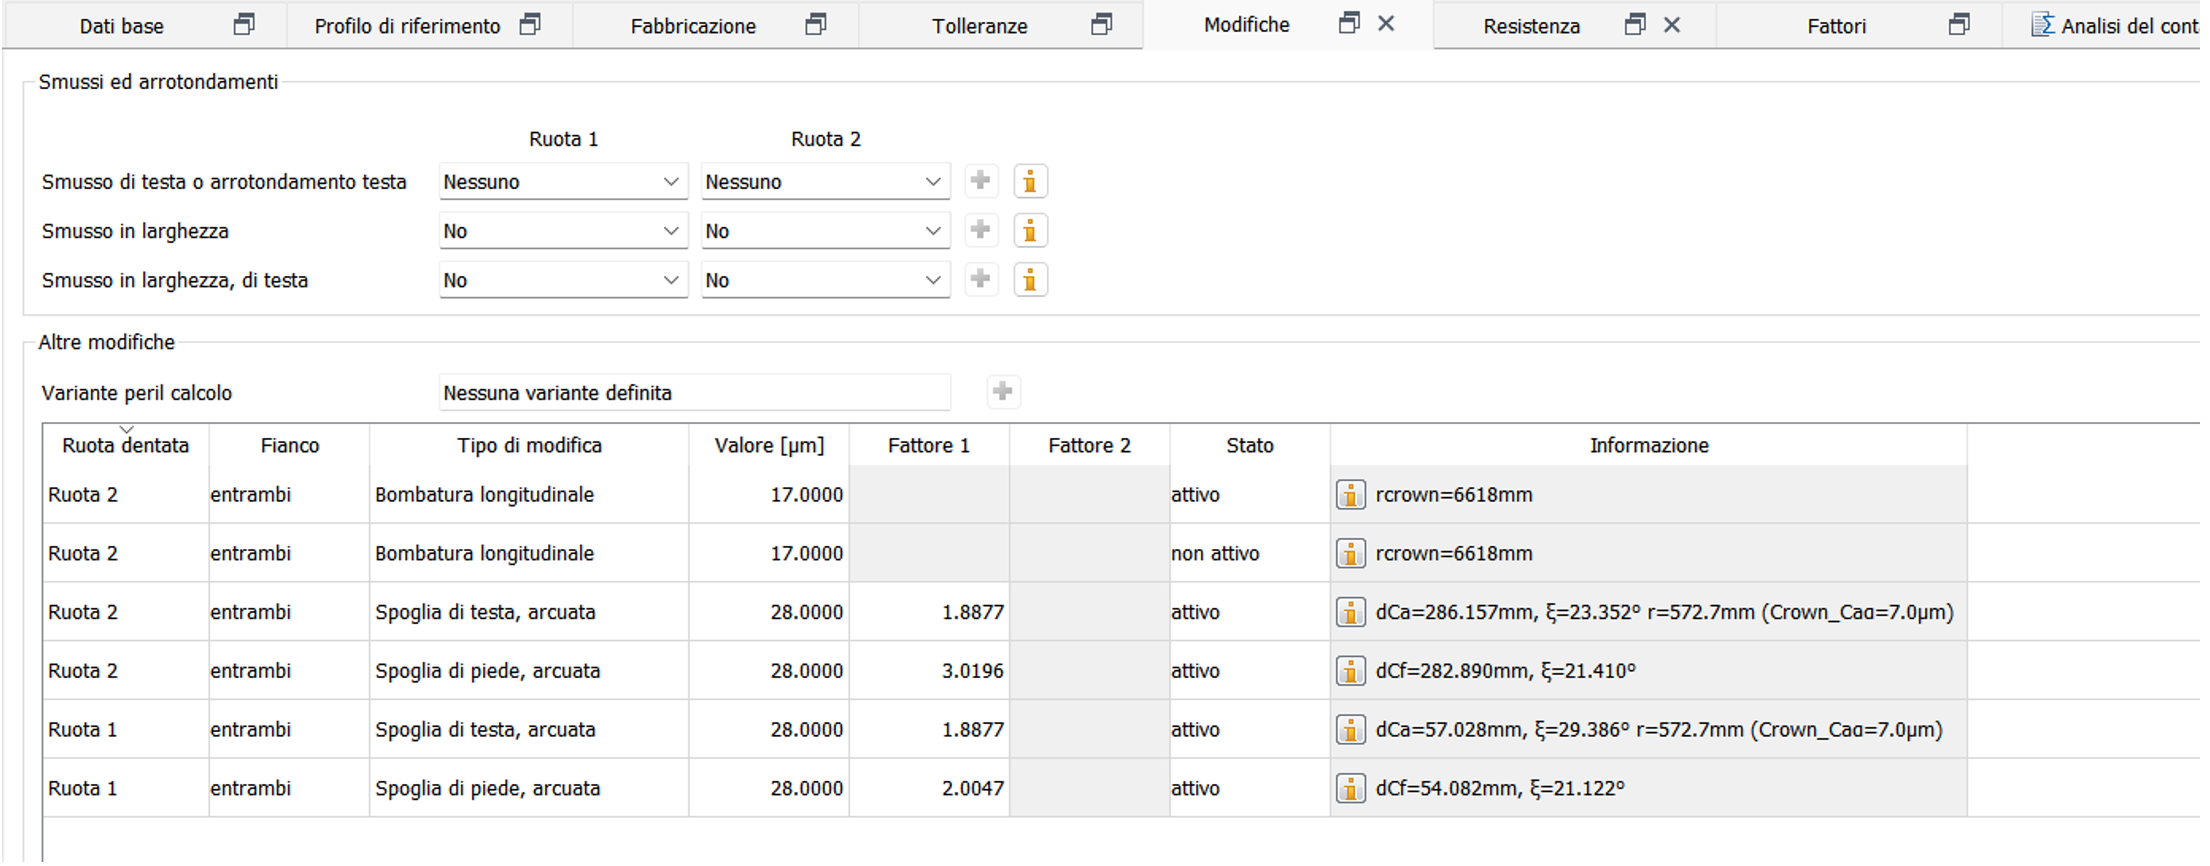
\includegraphics[scale=0.4]{Immagini/ModificheCoppia45.png}
    \caption{Modifiche delle ruote della coppia 4 5}
    \label{fig:ModificheCoppia45}
\end{figure}

Le modifiche effettuate sono state:
\begin{itemize}
    \item Ruota 1: spoglia di testa e di piede;
    \item Ruota 2: bombatura longitudinale, spoglia di testa e di piede.
\end{itemize}

Sezione \emph{Resistenza}
\begin{figure}[h]
    \centering
    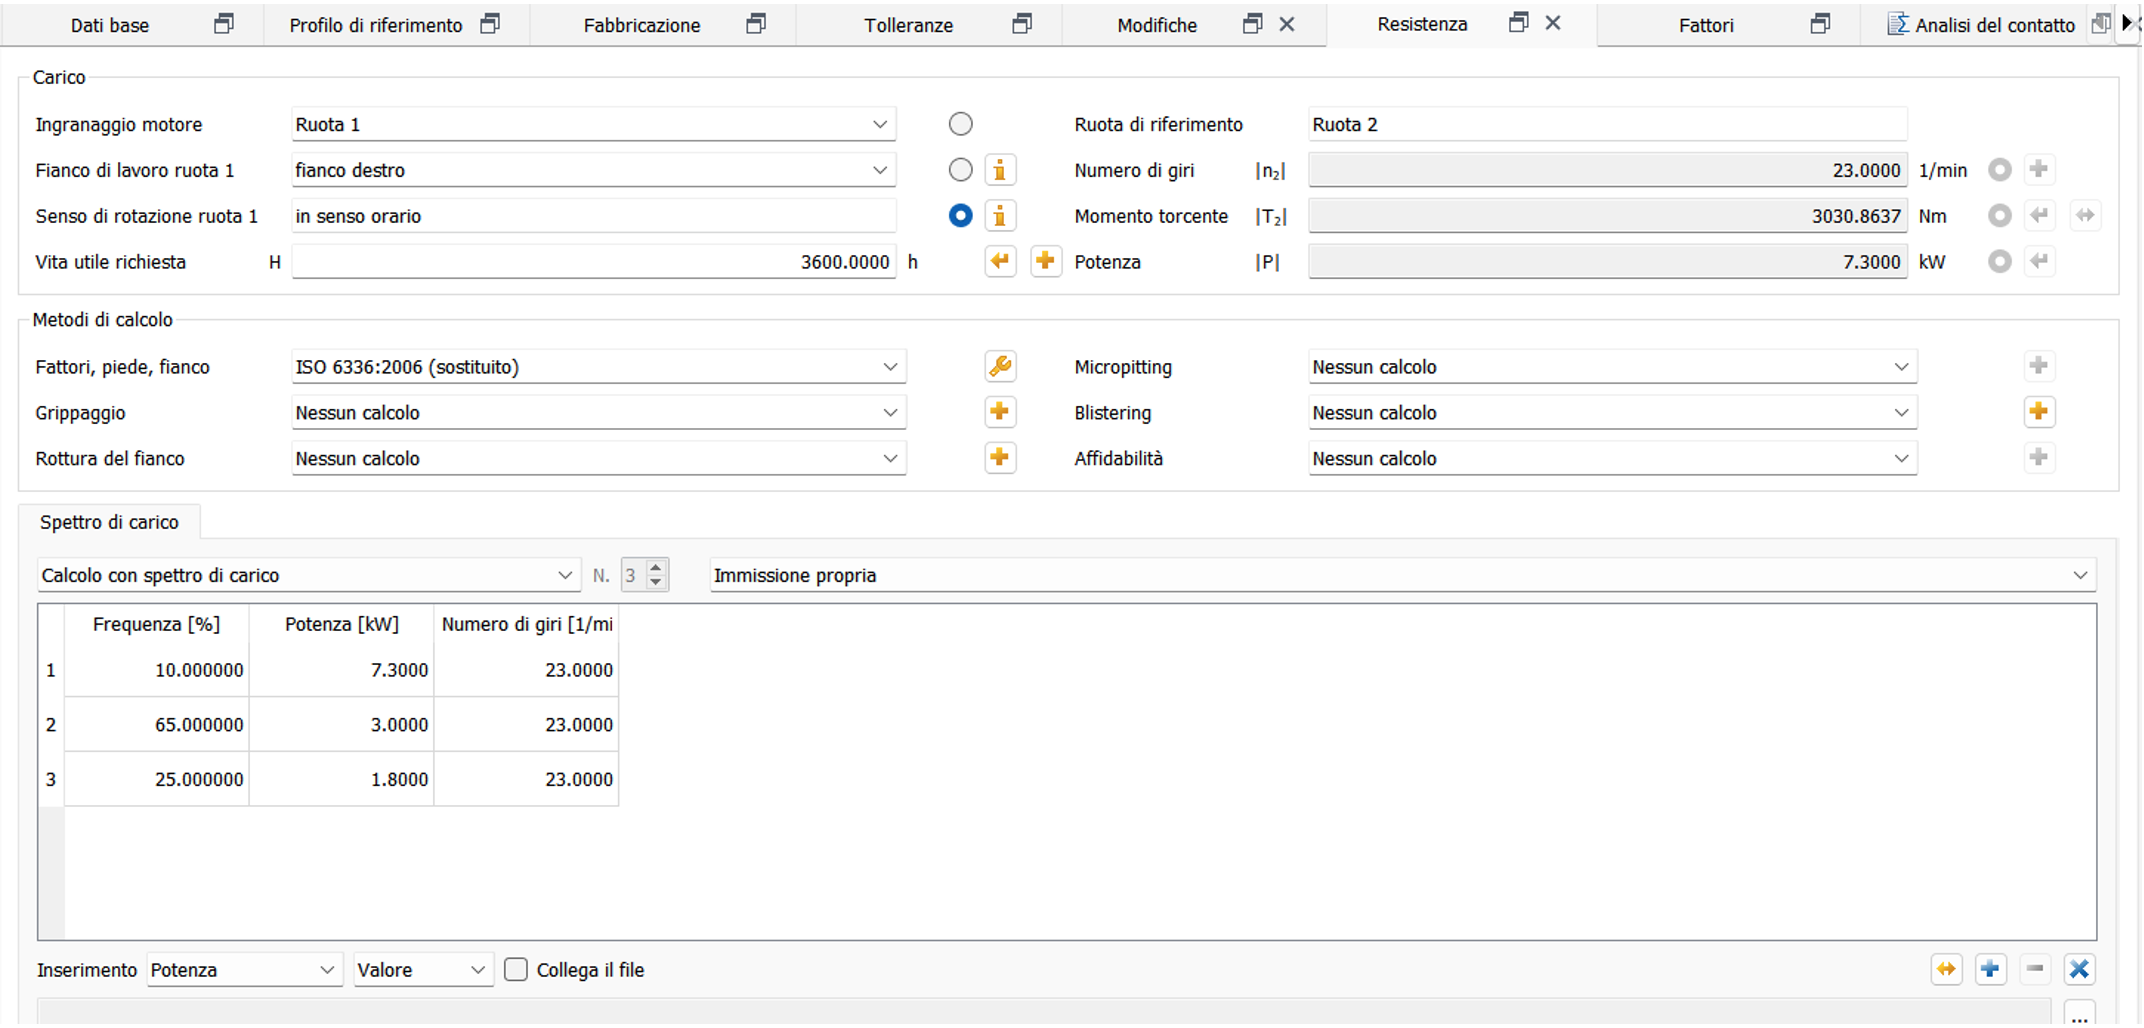
\includegraphics[scale=0.39]{Immagini/ResistenzaCoppia45.png}
    \caption{Resistenza delle ruote coppia 4 5}
    \label{fig:ResistenzaCoppia45}
\end{figure}

In questa sezione del software KissSoft vengono inserite Potenza, velocità e momento torcente funzionali al metodo di calcolo ISO6336:2006. La ruota di riferimento da selezionare è chiaramente la ruota motrice e si suppone che il fianco di lavorazione sia il destro. Inoltre, viene inserito manualmente il ciclo di carico fornito dai dati di progetto.
\newpage
Sezione \emph{Fattori}
\begin{figure}[h]
    \centering
    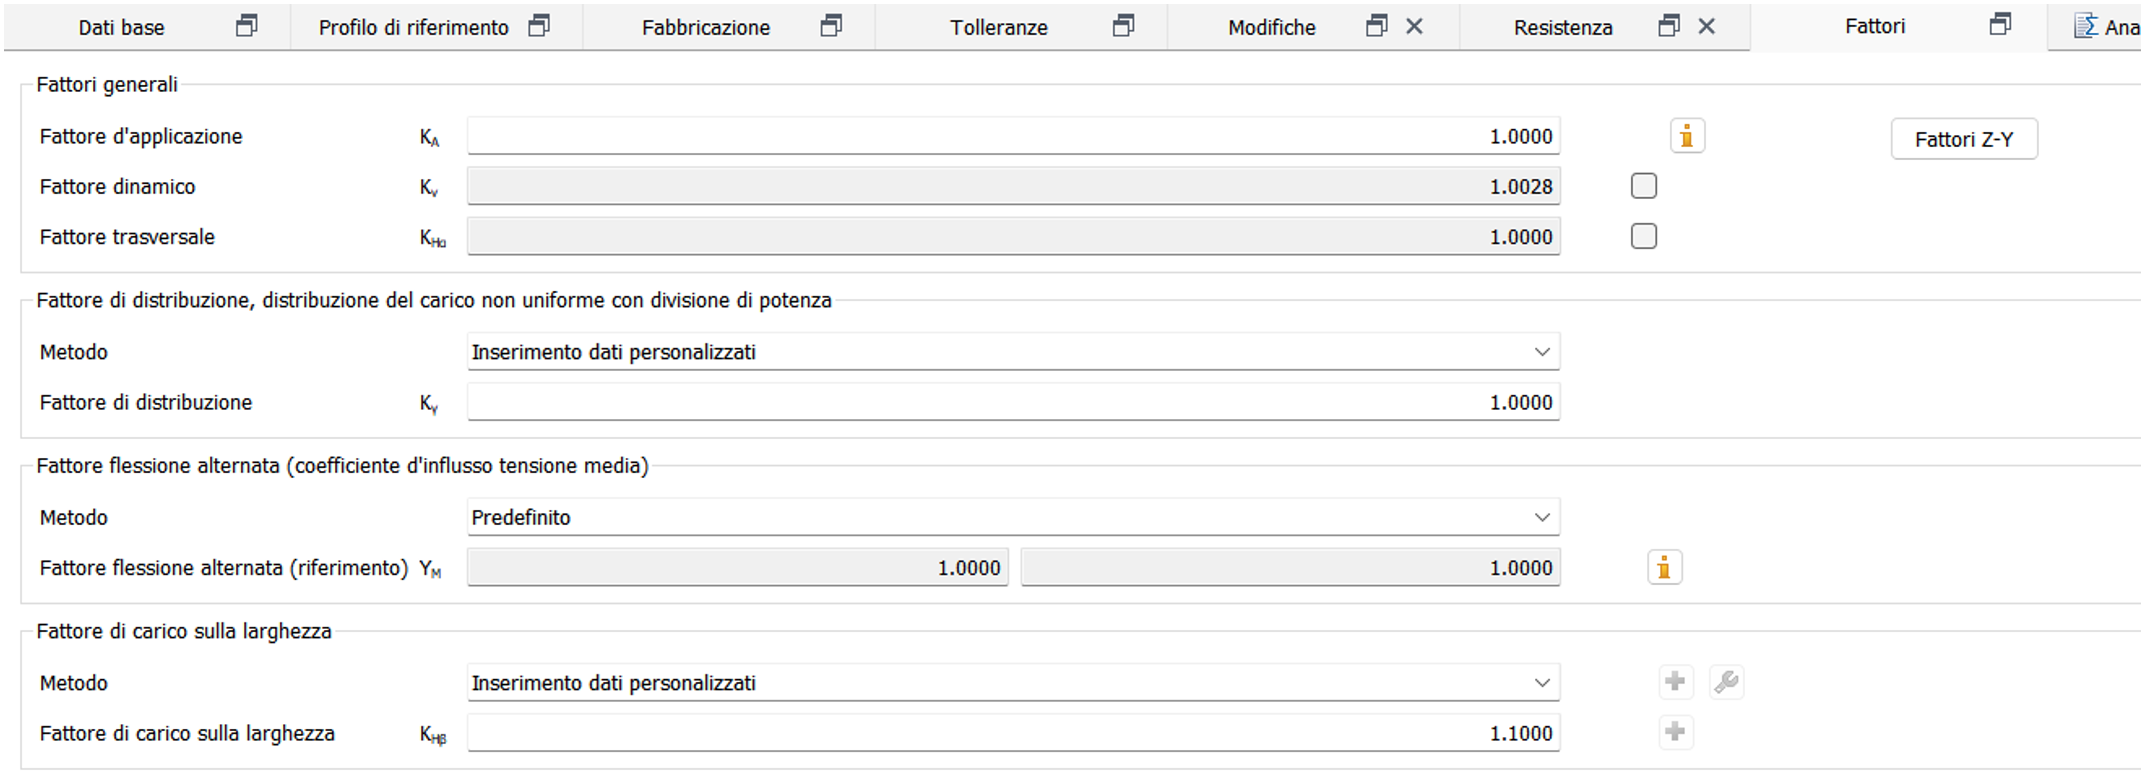
\includegraphics[scale=0.4]{Immagini/FattoriCoppia45.png}
    \caption{Fattori delle ruote della coppia 4 5}
    \label{fig:FattoriCoppia45}
\end{figure}

In questa sezione è stato ipotizzato un fattore di carico sulla lunghezza $K_{HB}$ pari a 1.1. Nel caso in questione albero e scatola sono elementi considerati rigidi, ma per fare un calcolo in sicurezza si suppone comunque che la pressione non sia distribuita in maniera perfettamente uniforme sul dente.\\
Il fattore di flessione alternata $Y_M$ è stato supposto 1, siccome si ha a che fare con un ciclo all’origine. Se si avesse avuto un ciclo alterno allora $Y_M$ sarebbe stato supposto pari a 0.7.\\
\\
Sezione \emph{Analisi del contatto}
\begin{figure}[h]
    \centering
    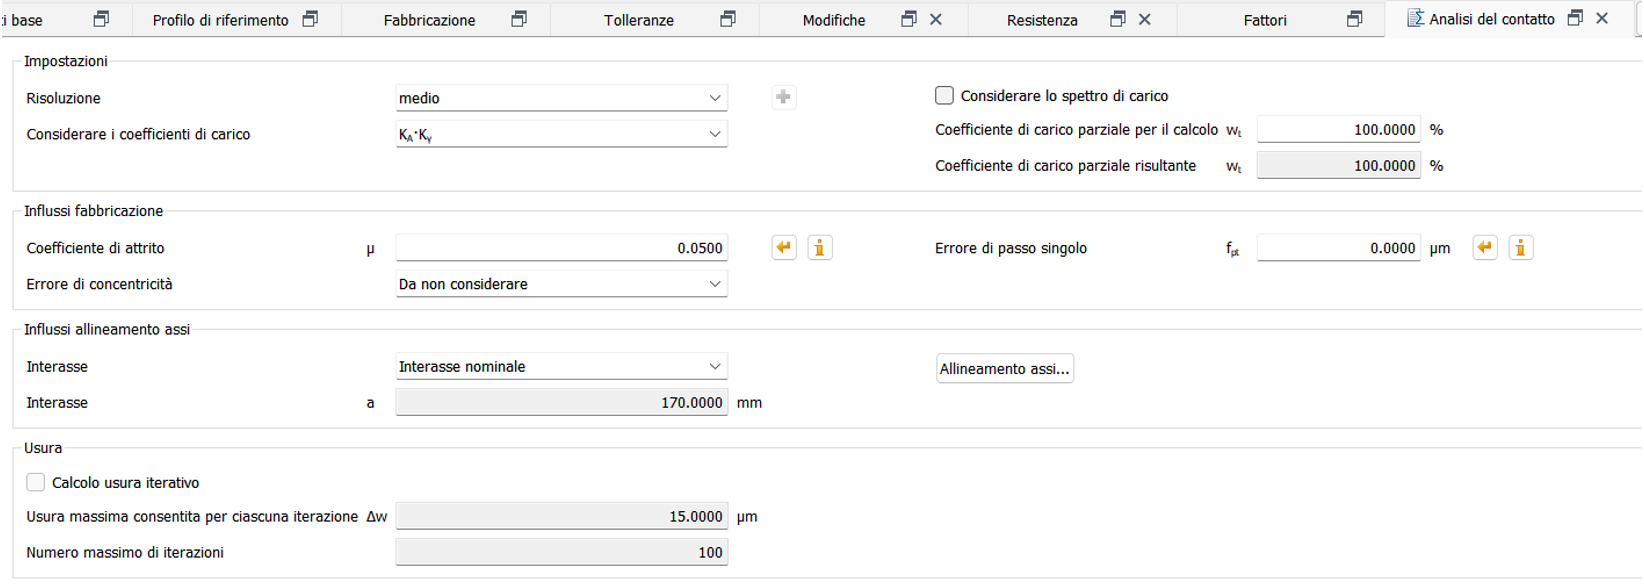
\includegraphics[scale=0.5]{Immagini/AnalisiContattoCoppia45.png}
    \caption{Analisi del contatto tra le ruote della coppia 4 5}
    \label{fig:AnalisiContattoCoppia45}
\end{figure}

In questa sezione del software si chiede a che carico si vuole far girare l’analisi di contatto in termini percentuali rispetto al valore del momento torcente che è stato inserito nella sezione “Resistenza”. Andando poi in "Grafica" è possibile vedere la Stress Distribution on Tooth 3D. \\
Se la situazione mostra una concentrazione delle tensioni molto accentuata a piede del dente è possibile andare a ri-modificare i fattori di "Modifiche" delle ruote.
\newpage
Ciò che è stato ottenuto in questa analisi è mostrato in Fig.\ref{fig:StressDistributionCoppia45}.
\begin{figure}[h]
    \centering
    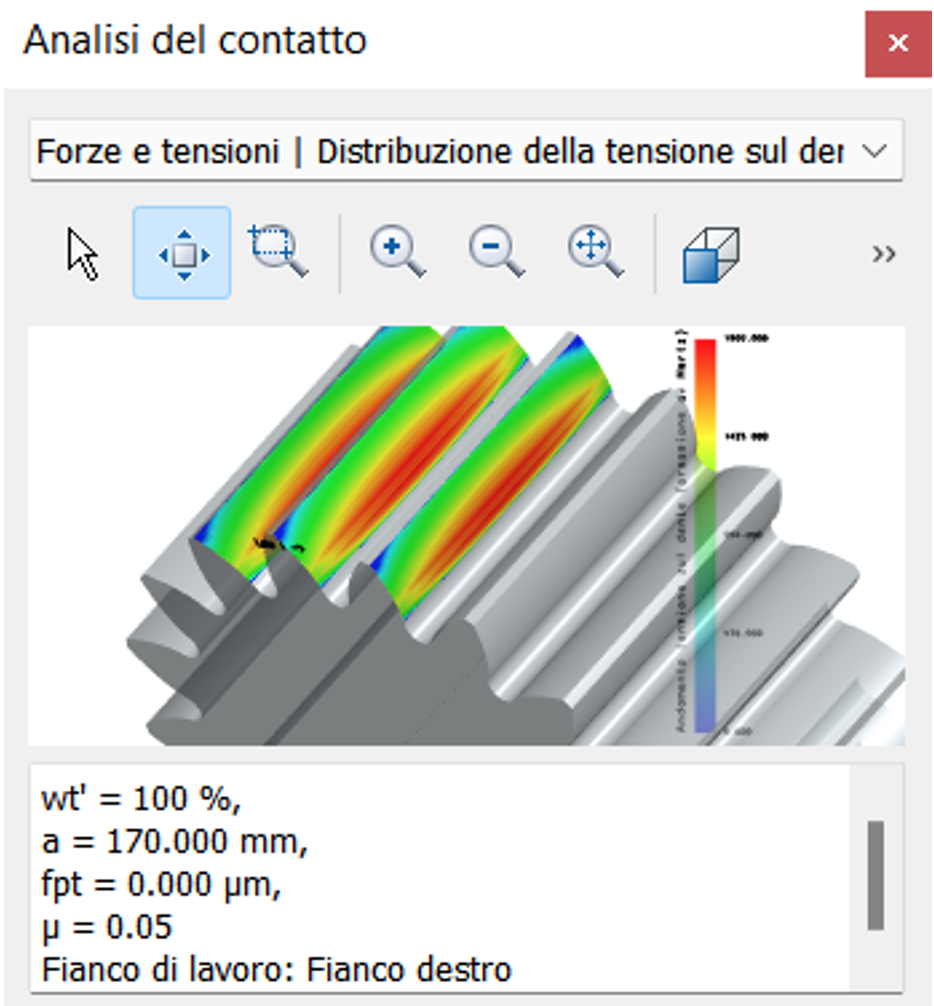
\includegraphics[scale=0.4]{Immagini/StressDistributionCoppia45.png}
    \caption{Andamento delle tensioni lungo il fianco del dente}
    \label{fig:StressDistributionCoppia45}
\end{figure}

La sollecitazione è concentrata sulla parte centrale del dente, soluzione ottimale per l’applicazione studiata. \\
Nella sezione "Risultati" è possibile visualizzare tutti i dati ottenuti dall’analisi (in particolare il fattore di ricoprimento e i valori dei coefficienti di sicurezza). \\
La verifica a resistenza risulta soddisfatta per i seguenti valori:
\begin{itemize}
    \item Sicurezza al piede del dente (Bending), $S_F>1.3$;
    \item Sicurezza al finaco del dente (Pitting), $S_H>1.1$.
    \end{itemize}
\begin{figure}[h]
    \centering
    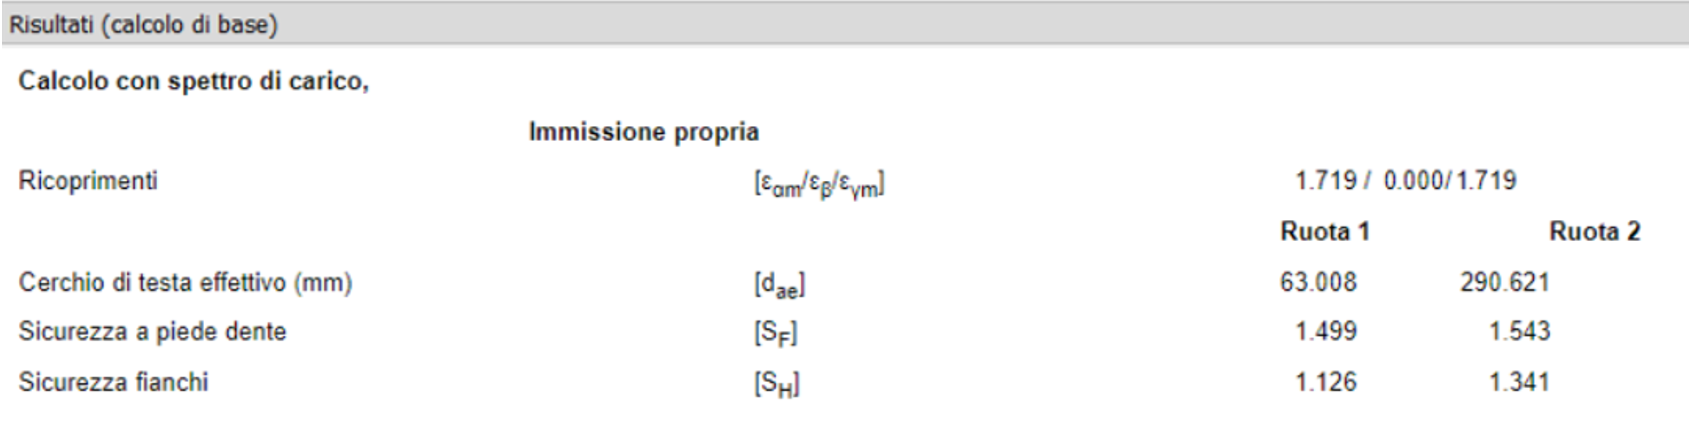
\includegraphics[scale=0.49]{Immagini/RisultatiCoppia45.png}
    \caption{Risultati dell'analisi del contatto tra le ruote della coppia 4 5}
    \label{fig:RisultatiCoppia45}
\end{figure}
\newpage
Il Software fornisce anche una rappresentazione 3D di massima dell’accoppiamento
\begin{figure}[h]
    \centering
    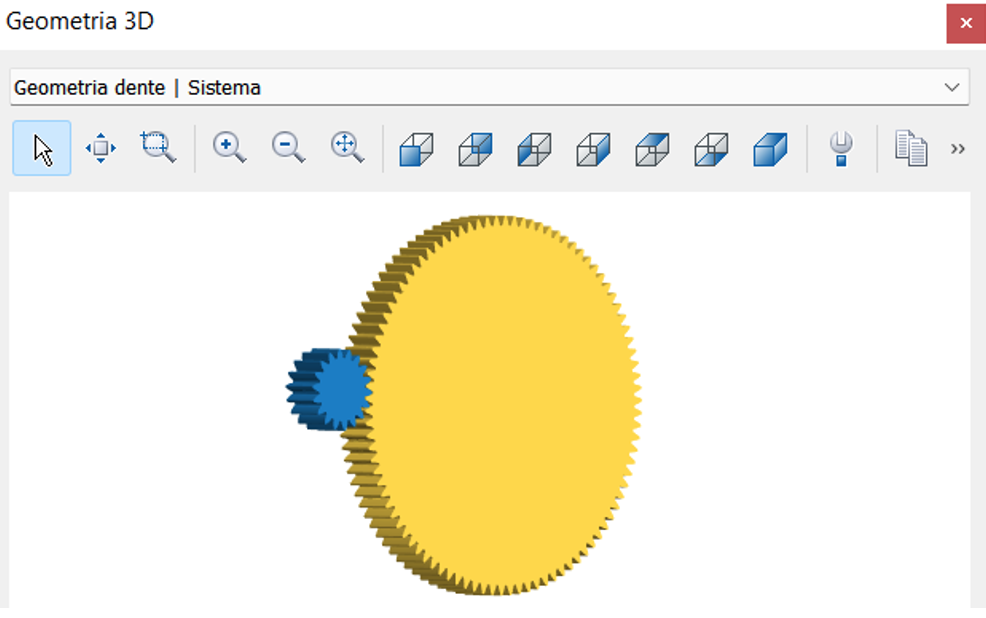
\includegraphics[scale=0.5]{Immagini/GeometriaCoppia45.png}
    \caption{Rappresentazione geometrica 3D della coppia di ruote 4 5}
    \label{fig:GeometriaCoppia45}
\end{figure}
\paragraph{Coppia cilindrica 6 7}
Definizione dei dati di base della coppia cilindrica:
\begin{figure}[h]
    \centering
    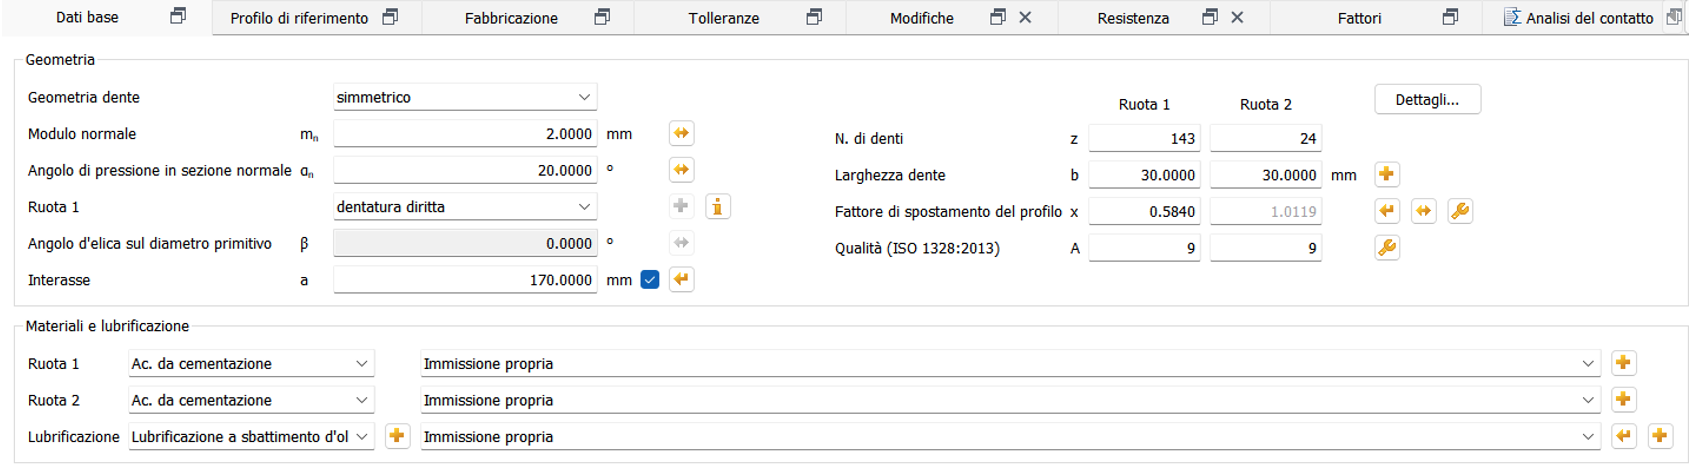
\includegraphics[scale=0.5]{Immagini/Coppia67.png}
    \caption{Dati di base coppia 6 7}
    \label{fig:Coppia67}
\end{figure}
\newpage
A seguito di diversi tentativi quindi per la seconda coppia cilindrica è stato scelto un numero di denti pari a 143 per la ruota 1 e pari a 24 per la ruota 2. Il modulo è stato supposto pari a 2 mm, la larghezza del dente pari a 30 mm, l’angolo di pressione $20^\circ$ e un interasse pari a 170 mm, ideale per rispettare gli ingombri disponibili. 
La qualità degli ingranaggi pari a 9 (ISO1328), mentre il materiale scelto per entrambe le ruote è un acciaio da cementazione 20MnCr5, con un carico di rottura $R_m$ pari a $1200\ N/mm^2$ e un carico di snervamento $R_s$ pari a $850\ N/mm^2$. 
\begin{figure}[h]
    \centering
    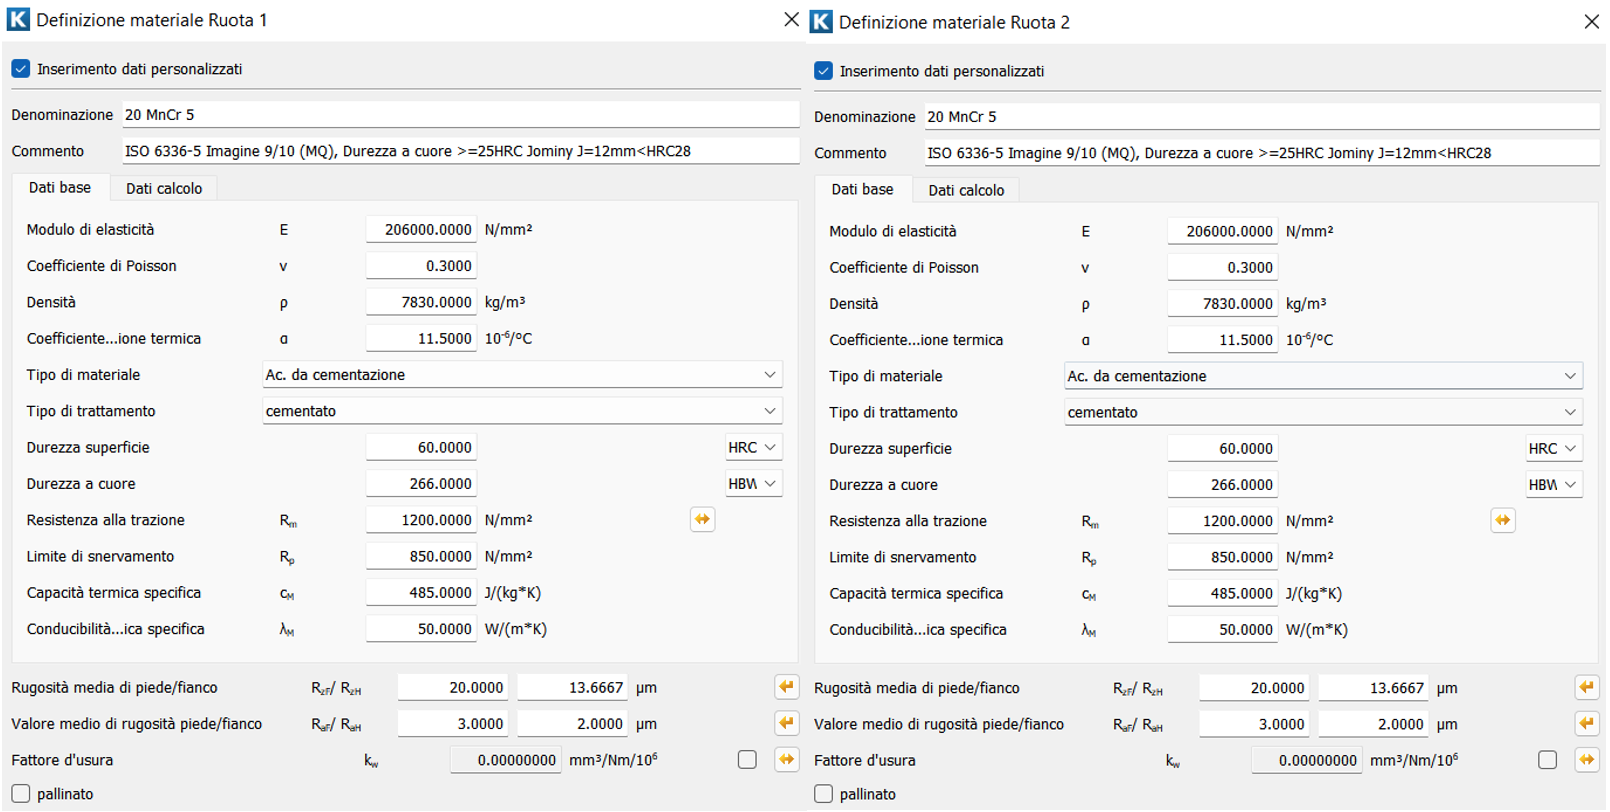
\includegraphics[scale=0.5]{Immagini/RuoteCoppia67.png}
    \caption{Parametri delle ruote della coppia 6 7}
    \label{fig:RuoteCoppia45}
\end{figure}

Per quanto riguarda il lubrificante invece non essendo presente tra le scelte del software è stato necessario crearlo procedendo come in Fig.\ref{fig:LubrificanteCoppia45}, inserendo tutti i dati di progetto richiesti. Il lubrificante utilizzato è lo \textit{SPIRAX S3 AX 80W-90}, con le seguenti caratteristiche: 
\begin{figure}[h]
    \centering
    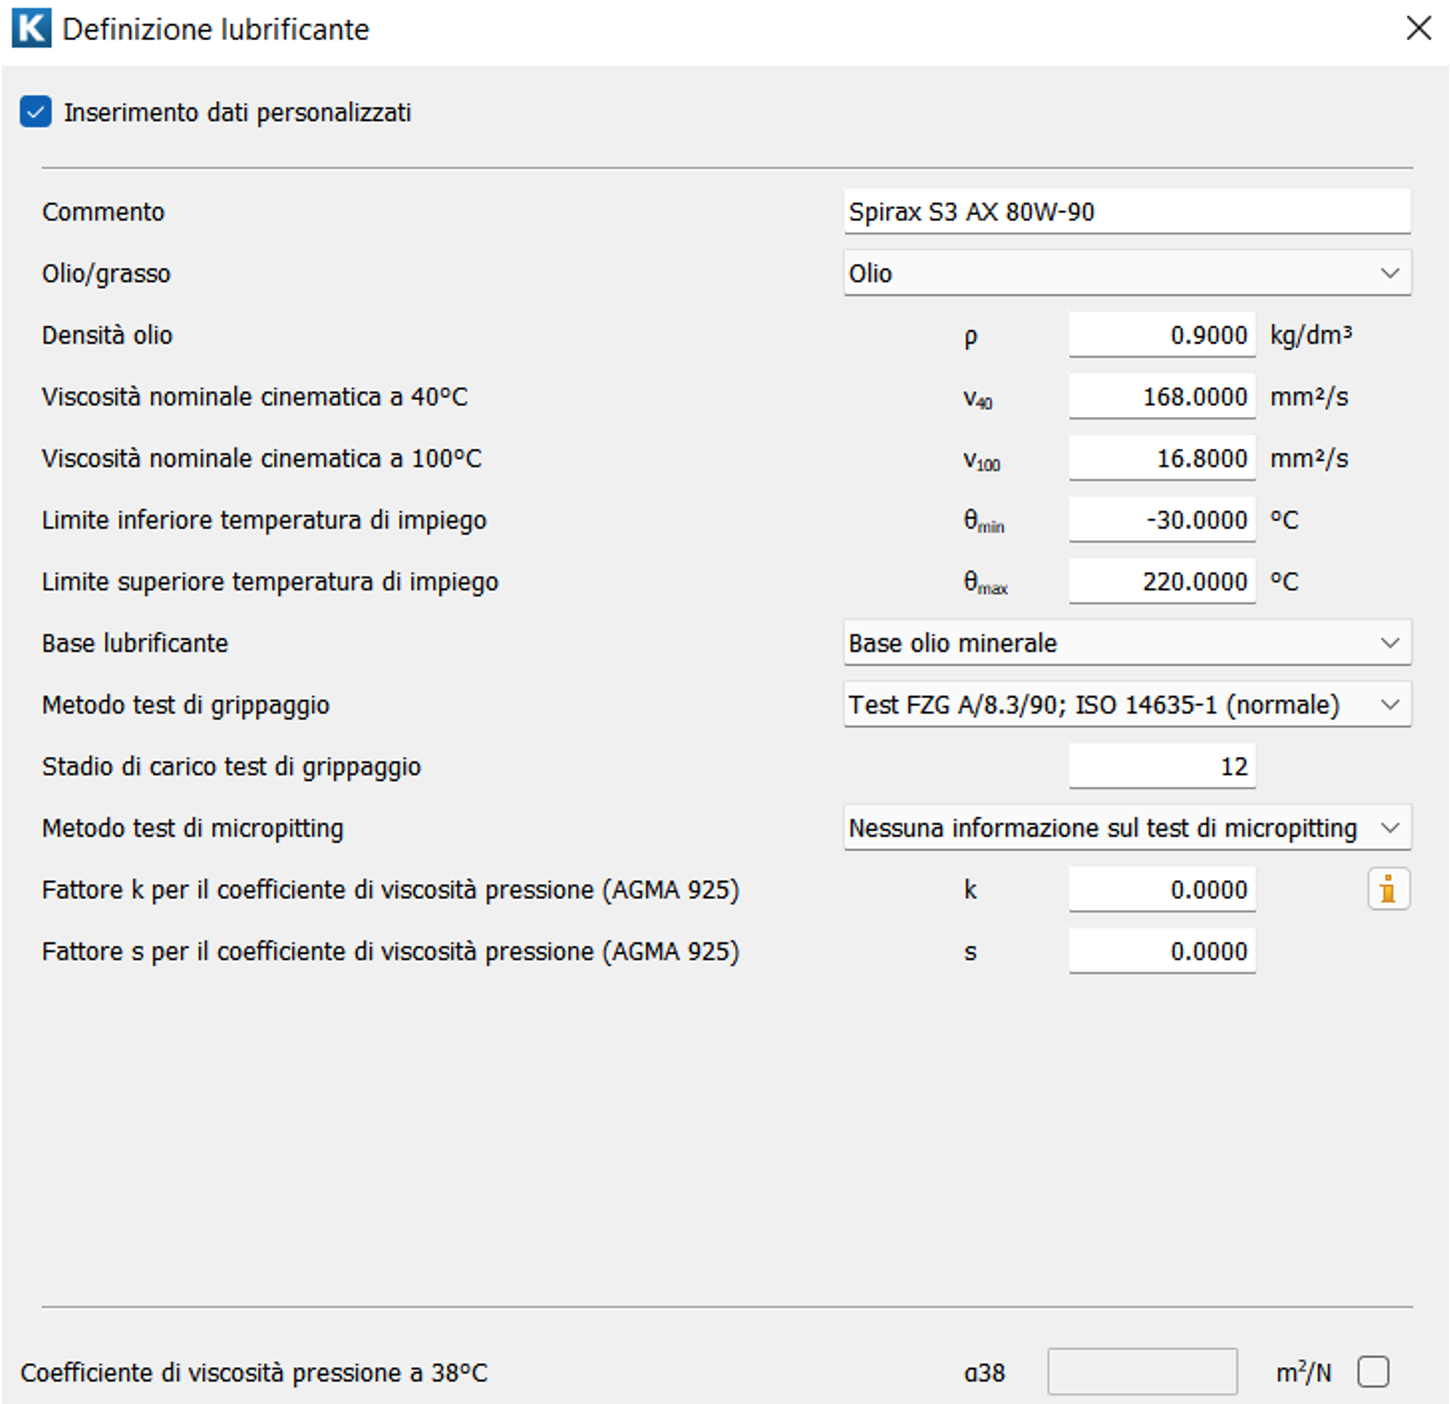
\includegraphics[scale=0.35]{Immagini/LubrificanteCoppia45.png}
    \caption{Parametri caratteristici del lubrificante}
    \label{fig:LubrificanteCoppia45}
\end{figure}

Le altre sezioni del KissSoft per la prima coppia cilindrica sono state così compilate.\\
\\
Sezione \emph{Profilo di riferimento}
\begin{figure}[h]
    \centering
    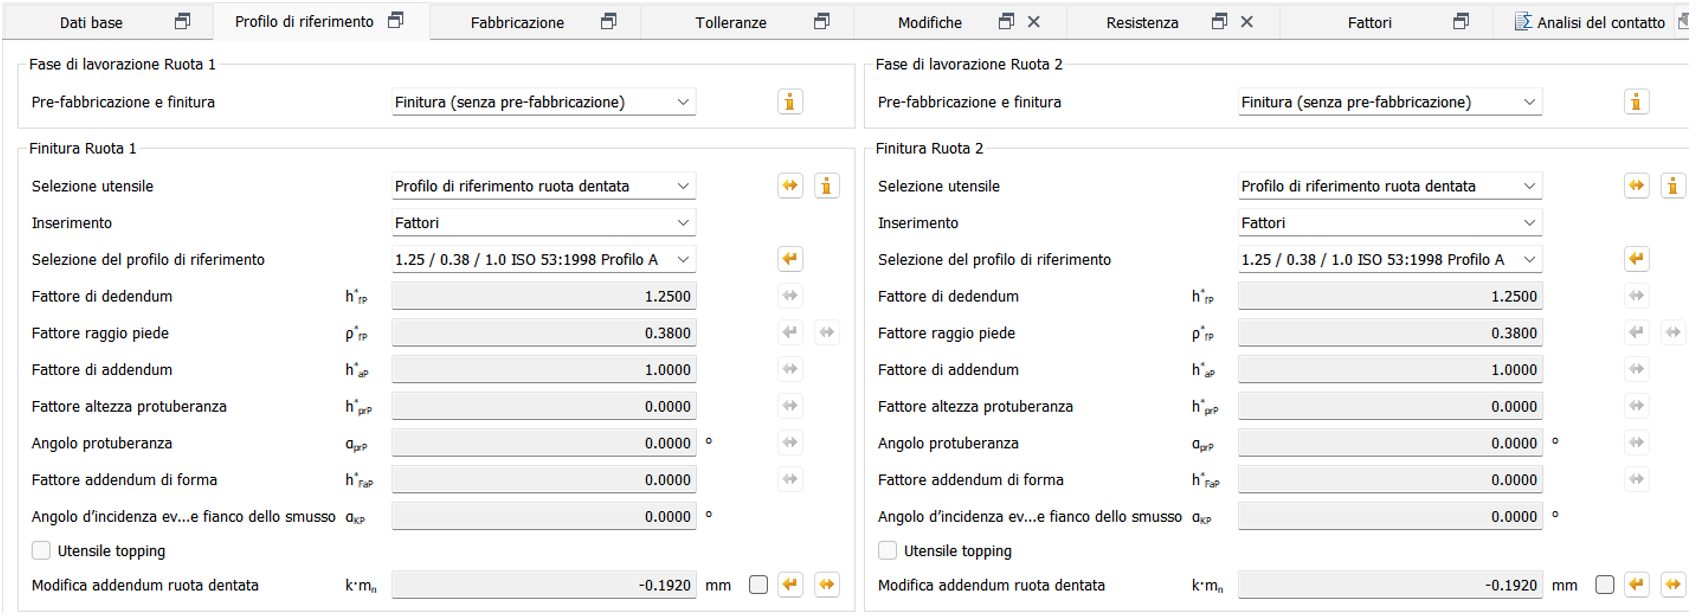
\includegraphics[scale=0.5]{Immagini/ProfiloRiferimentoCoppia67.png}
    \caption{Profilo di riferimento delle due ruote della coppia 6 7}
    \label{fig:ProfiloRiferimentoCoppia67}
\end{figure}

Questa sezione riguarda il tipo di profilo utensile utilizzato per l’inviluppo del dente. 
In generale per ruote standard si utilizza o prefabbricazione o finitura (senza prefabbricazione), come nel caso in esame. Una volta scelto il profilo di riferimento i dati vengo inseriti in automatico dal Software.\\

Sezione \emph{Fabbricazione}
\begin{figure}[h]
    \centering
    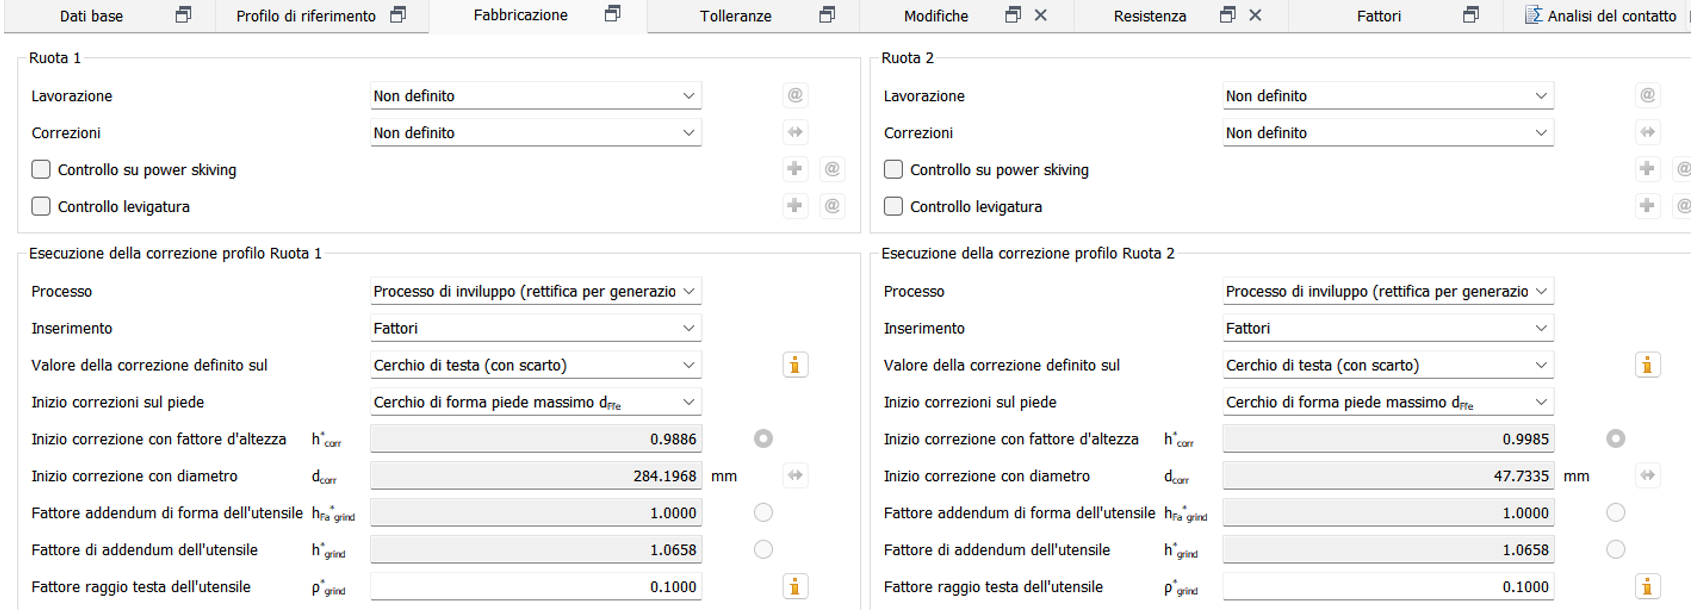
\includegraphics[scale=0.5]{Immagini/FabbricazioneCoppia67.png}
    \caption{Parametri di fabbricazione delle ruote della coppia 6 7}
    \label{fig:FabbricazioneCoppia67}
\end{figure}
\newpage
Sezione \emph{Tolleranze}
\begin{figure}[h]
    \centering
    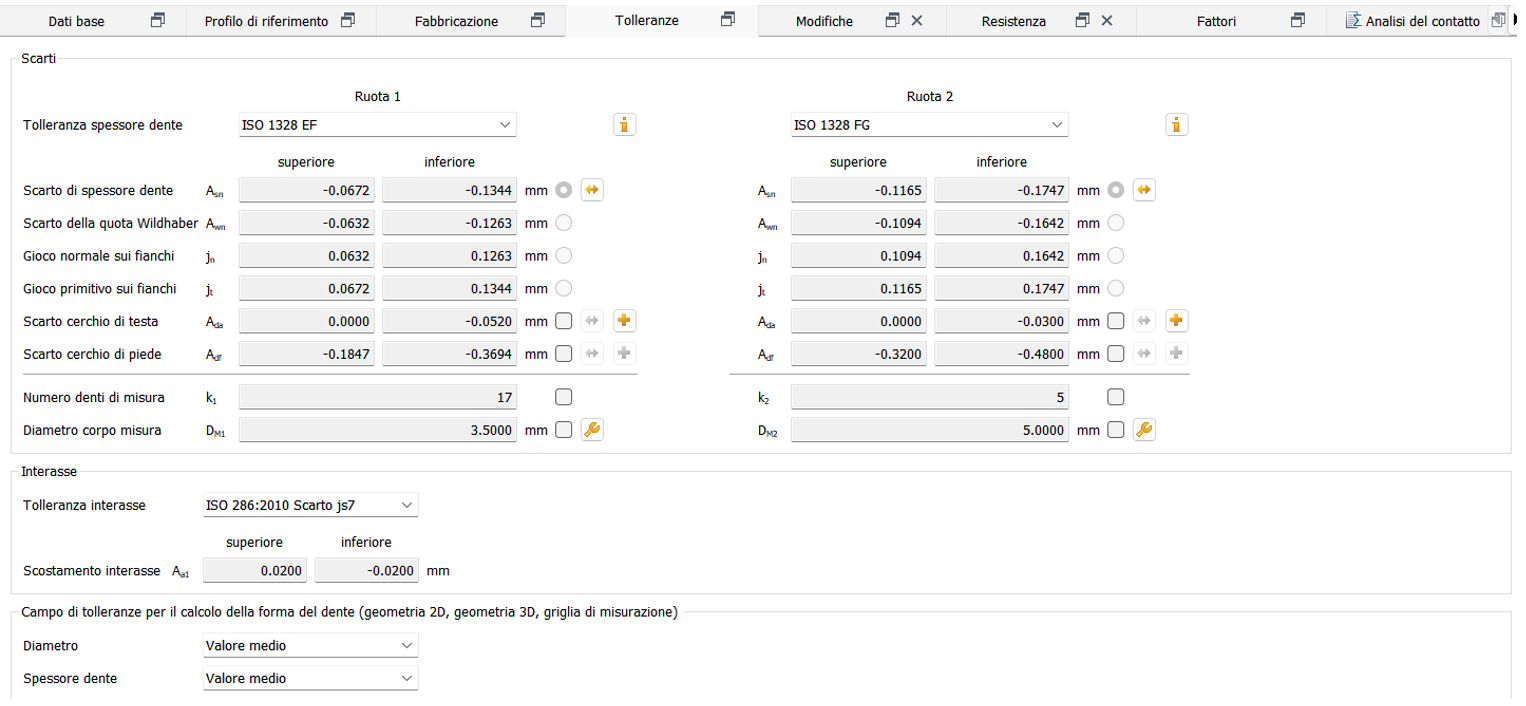
\includegraphics[scale=0.5]{Immagini/TolleranzeCoppia67.png}
    \caption{Tolleranze delle ruote della coppia 6 7}
    \label{fig:TolleranzeCoppia67}
\end{figure}

Questa sezione permette di inserire le diverse tolleranze relative agli scarti e interasse, all’interno di “Scarti” compare la voce “Tolleranza spessore dente” dove è stata scelta la tipologia di tolleranza in base alla normativa ISO1328. Per quanto riguarda la tolleranza all’interasse è stata scelta la voce ISO 286:2010 Scarto js7.\\
Le tolleranze non sono importanti per la parte di calcolo dell’ingranaggio, ma sono funzionali al disegno. La tolleranza più importante è quella della testa del dente, funzionale per la fase di tornitura. \\
\\
Sezione \emph{Modifiche}
\begin{figure}[h]
    \centering
    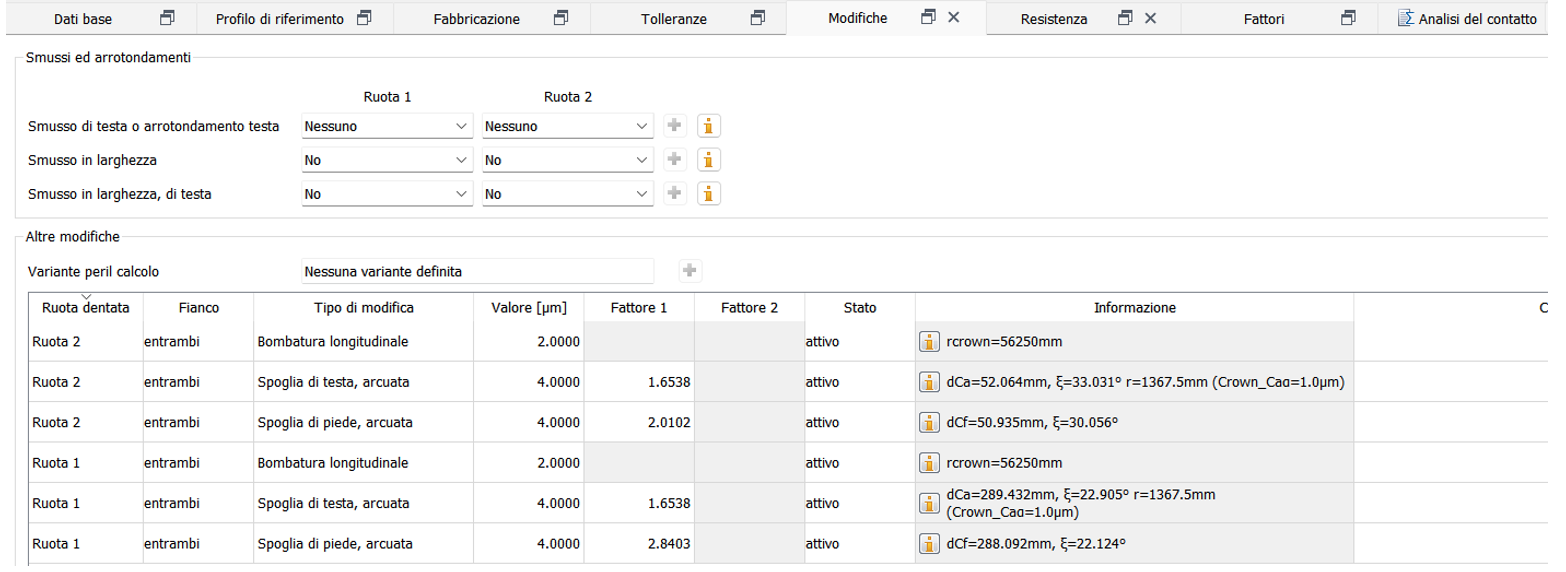
\includegraphics[scale=0.5]{Immagini/ModificheCoppia67.png}
    \caption{Modifiche delle ruote della coppia 6 7}
    \label{fig:ModificheCoppia67}
\end{figure}

Le modifiche effettuate sono state:
\begin{itemize}
    \item Ruota 1: bombatura longitudinale, spoglia di testa e di piede;
    \item Ruota 2: bombatura longitudinale, spoglia di testa e di piede.
\end{itemize}
\newpage
Sezione \emph{Resistenza}
\begin{figure}[h]
    \centering
    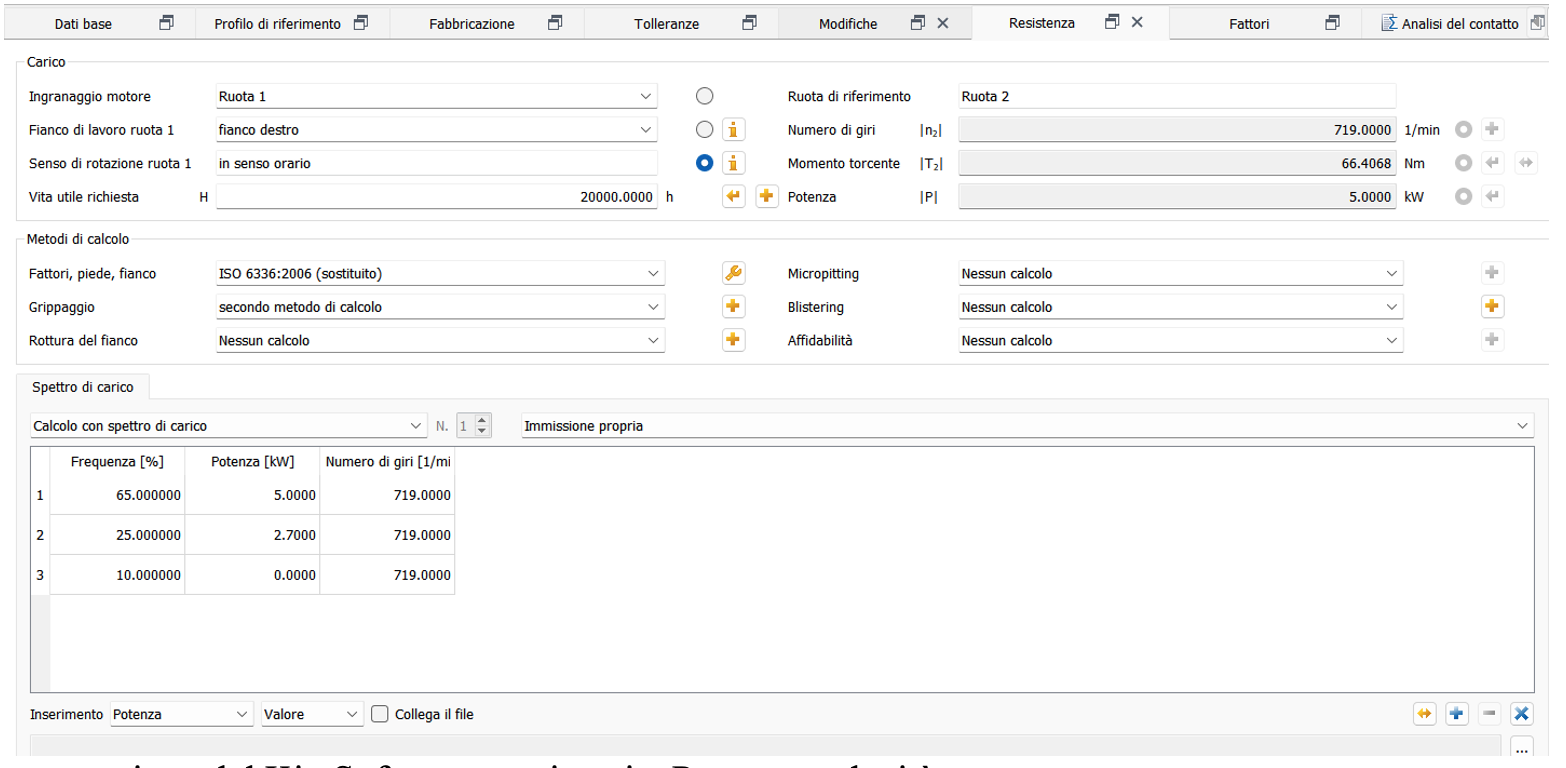
\includegraphics[scale=0.5]{Immagini/ResistenzaCoppia67.png}
    \caption{Resistenza delle ruote coppia 6 7}
    \label{fig:ResistenzaCoppia67}
\end{figure}

In questa sezione del software KissSoft vengono inserite Potenza, velocità e momento torcente funzionali al metodo di calcolo ISO6336:2006. La ruota di riferimento da selezionare è chiaramente la ruota motrice e si suppone che il fianco di lavorazione sia il destro. Inoltre, viene inserito manualmente il ciclo di carico fornito dai dati di progetto.\\
\\
Sezione \emph{Fattori}
\begin{figure}[h]
    \centering
    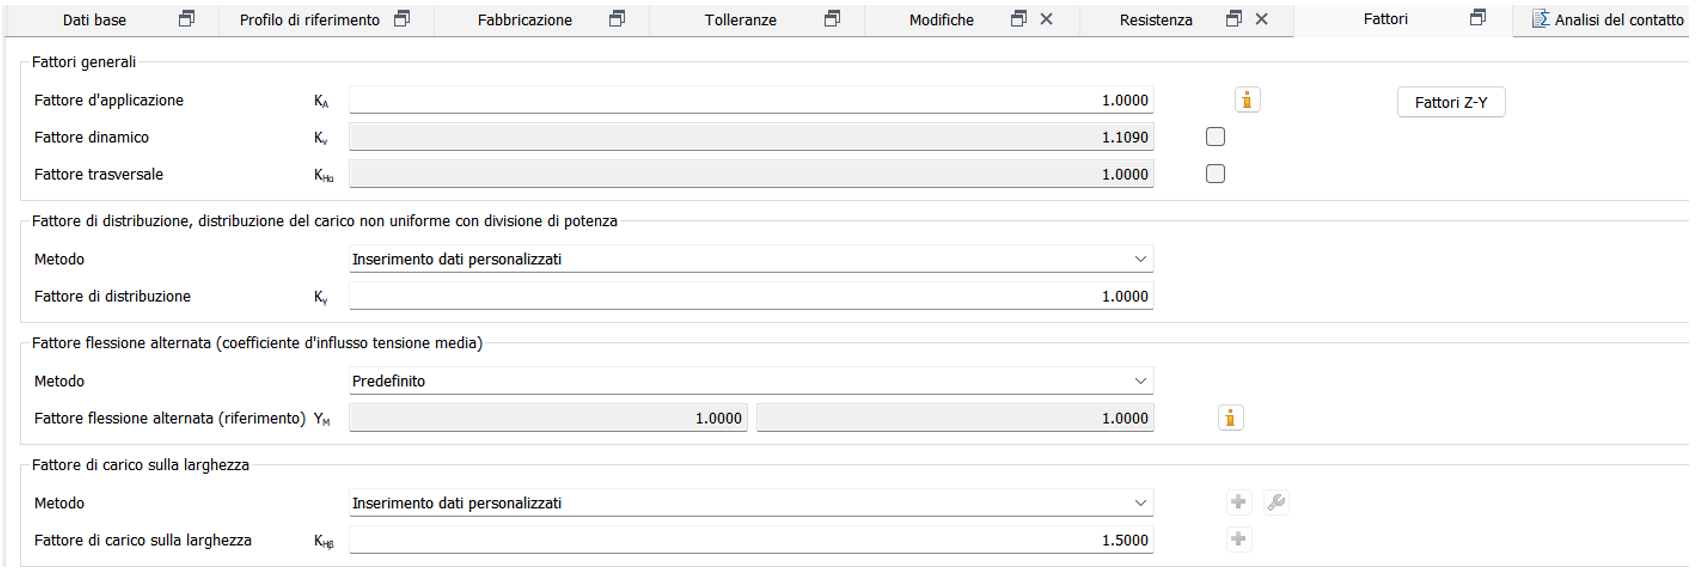
\includegraphics[scale=0.5]{Immagini/FattoriCoppia67.png}
    \caption{Fattori delle ruote della coppia 6 7}
    \label{fig:FattoriCoppia67}
\end{figure}

In questa sezione è stato ipotizzato un fattore di carico sulla lunghezza $K_{HB}$ pari a 1.5. Nel caso in questione albero e scatola sono elementi considerati rigidi, ma per fare un calcolo in sicurezza si suppone comunque che la pressione non sia distribuita in maniera perfettamente uniforme sul dente.\\
Il fattore di flessione alternata $Y_M$ è stato supposto 1, siccome si ha a che fare con un ciclo all’origine. Se si avesse avuto un ciclo alterno allora $Y_M$ sarebbe stato supposto pari a 0.7.
\newpage
Sezione \emph{Analisi del contatto}
\begin{figure}[h]
    \centering
    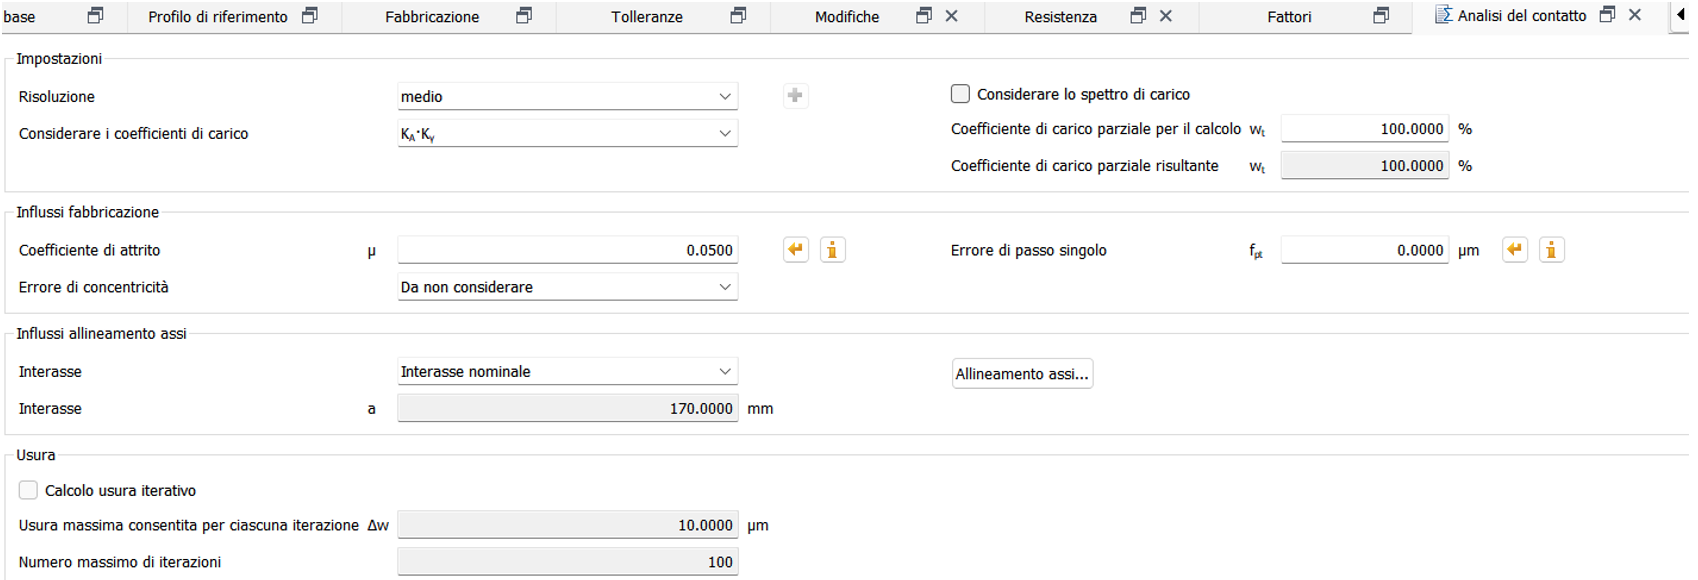
\includegraphics[scale=0.5]{Immagini/AnalisiContattoCoppia67.png}
    \caption{Analisi del contatto tra le ruote della coppia 6 7}
    \label{fig:AnalisiContattoCoppia67}
\end{figure}

In questa sezione del software si chiede a che carico si vuole far girare l’analisi di contatto in termini percentuali rispetto al valore del momento torcente che è stato inserito nella sezione “Resistenza”. Andando poi in "Grafica" è possibile vedere la Stress Distribution on Tooth 3D. \\
Se la situazione mostra una concentrazione delle tensioni molto accentuata a piede del dente è possibile andare a ri-modificare i fattori di "Modifiche" delle ruote.\\
\\
Ciò che è stato ottenuto in questa analisi è mostrato in Fig.\ref{fig:StressDistributionCoppia67}.
\begin{figure}[h]
    \centering
    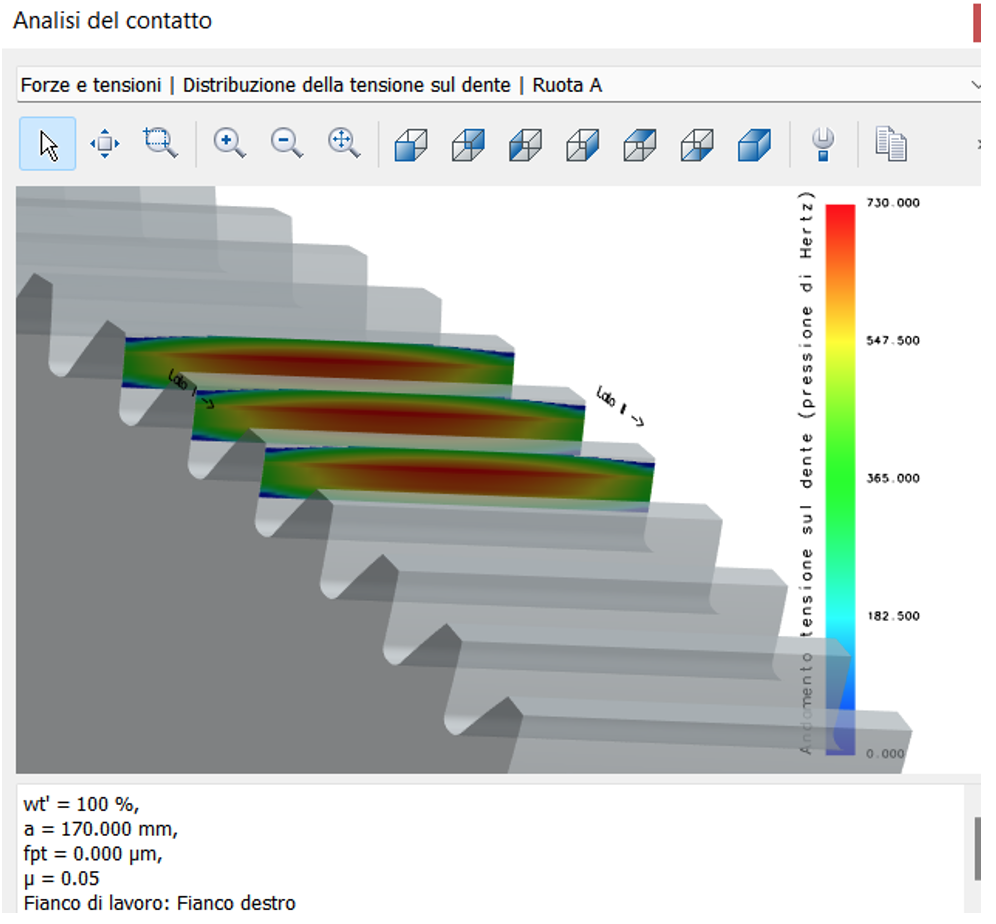
\includegraphics[scale=0.4]{Immagini/StressDistributionCoppia67.png}
    \caption{Andamento delle tensioni lungo il fianco del dente}
    \label{fig:StressDistributionCoppia67}
\end{figure}

La sollecitazione è concentrata sulla parte centrale del dente, soluzione ottimale per l’applicazione studiata. 
\newpage
Nella sezione "Risultati" è possibile visualizzare tutti i dati ottenuti dall’analisi (in particolare il fattore di ricoprimento e i valori dei coefficienti di sicurezza). \\
La verifica a resistenza risulta soddisfatta per i seguenti valori:
\begin{itemize}
    \item Sicurezza al piede del dente (Bending), $S_F>1.3$;
    \item Sicurezza al fianco del dente (Pitting), $S_H>1.1$.
    \end{itemize}
\begin{figure}[h]
    \centering
    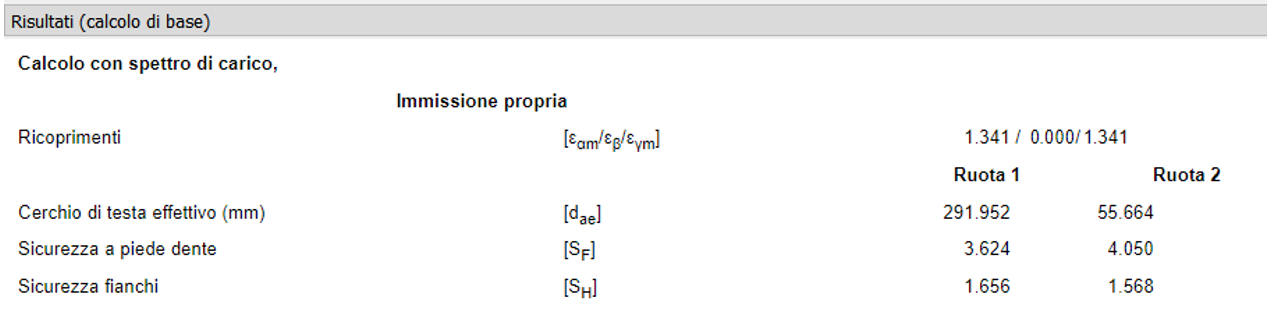
\includegraphics[scale=0.6]{Immagini/RisultatiCoppia67.png}
    \caption{Risultati dell'analisi del contatto tra le ruote della coppia 6 7}
    \label{fig:RisultatiCoppia67}
\end{figure}

Il Software fornisce anche una rappresentazione 3D di massima dell’accoppiamento
\begin{figure}[h]
    \centering
    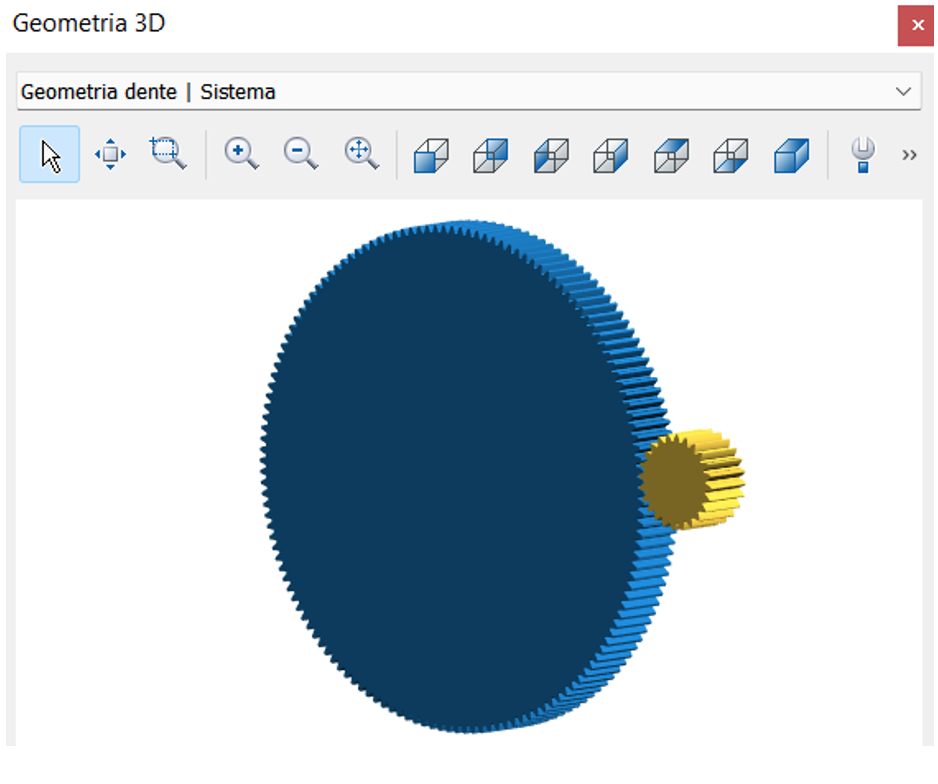
\includegraphics[scale=0.5]{Immagini/GeometriaCoppia67.png}
    \caption{Rappresentazione geometrica 3D della coppia di ruote 6 7}
    \label{fig:GeometriaCoppia67}
\end{figure}
\subsubsection{Dimensionamento coppie coniche}
\paragraph{Metodologia aapplicata per il dimensionamento}
Per la definizione della geometria si è utilizzato il diametro primitivo della seconda ruota oppure il modulo. Una volta scelto questo, si è inserito il numero di denti esatto ottenuto anche questa volta attraverso calcoli iterativi (sempre rispettando il rapporto di trasmissione e utilizzando il foglio di calcolo Excel), esattamente come fatto per le coppie cilindriche. 
Si è scelto infatti modulo e numero di denti che fornissero un diametro primitivo che rispettasse gli ingombri imposti dai dati di progetto e si è supposto poi un angolo di pressione pari a $20^\circ$. Si è infine scelta la tipologia di dentatura, in entrambe le coppie coniche dritta. L’angolo tra gli assi considerato è sempre $90^\circ$. 
\newpage
\paragraph{Coppia conica 0 1}Definizione dei dati di base della coppia conica.  
\begin{figure}[h]
    \centering
    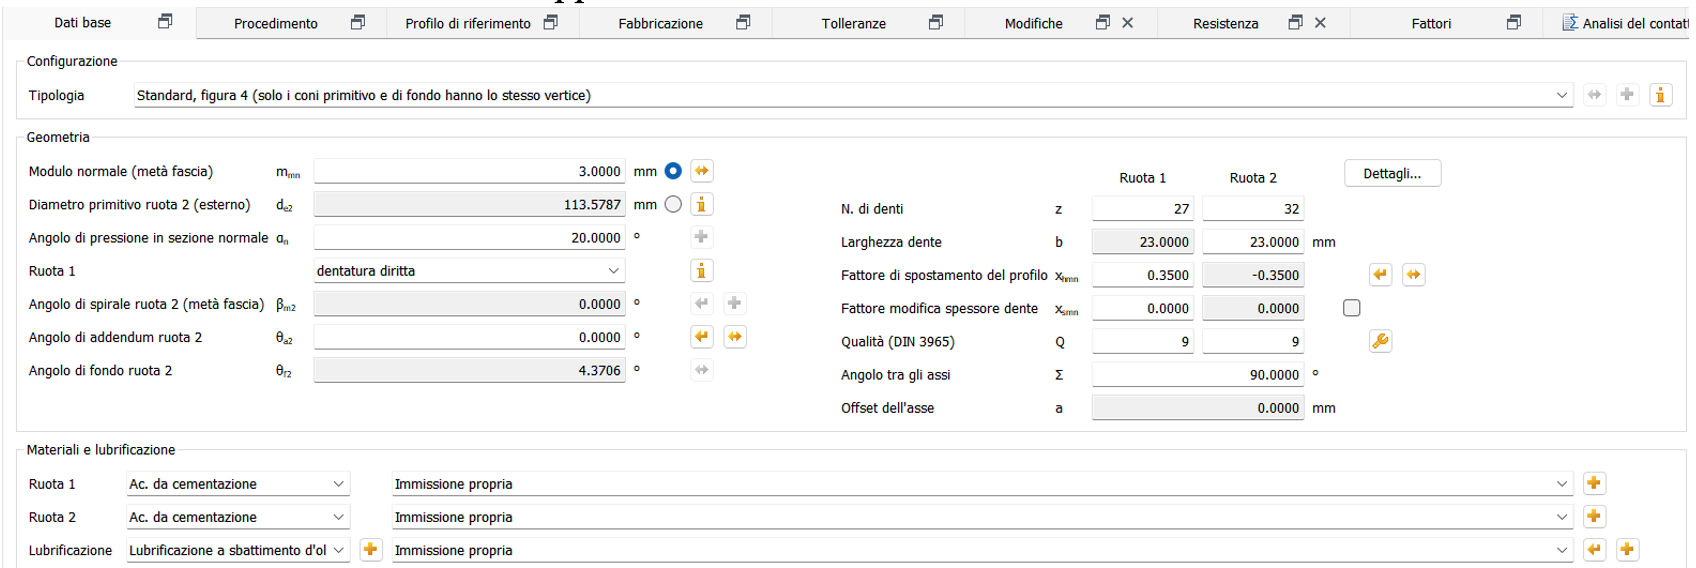
\includegraphics[scale=0.47]{Immagini/Coppia01.png}
    \caption{Dati di base coppia 0 1}
    \label{fig:Coppia01}
\end{figure}

A seguito di diversi tentativi quindi per la prima coppia conica è stato scelto un numero di denti pari a 27 per la ruota 1 e pari a 32 per la ruota 2. Il modulo è stato supposto pari a 3 mm, la larghezza del dente pari a 23 mm, l’angolo di pressione $20^\circ$ e un diametro primitivo della seconda ruota pari a 114 mm, ideale per rispettare gli ingombri disponibili. La qualità degli ingranaggi pari a 9 (DIN3965). Il materiale scelto per entrambe le ruote è un acciaio da cementazione 20MnCr5, con un carico di rottura $R_m$ pari a $1200\ N/mm^2$ e un carico di snervamento $R_s$ pari a 850 $N/mm^2$. 
\begin{figure}[h]
    \centering
    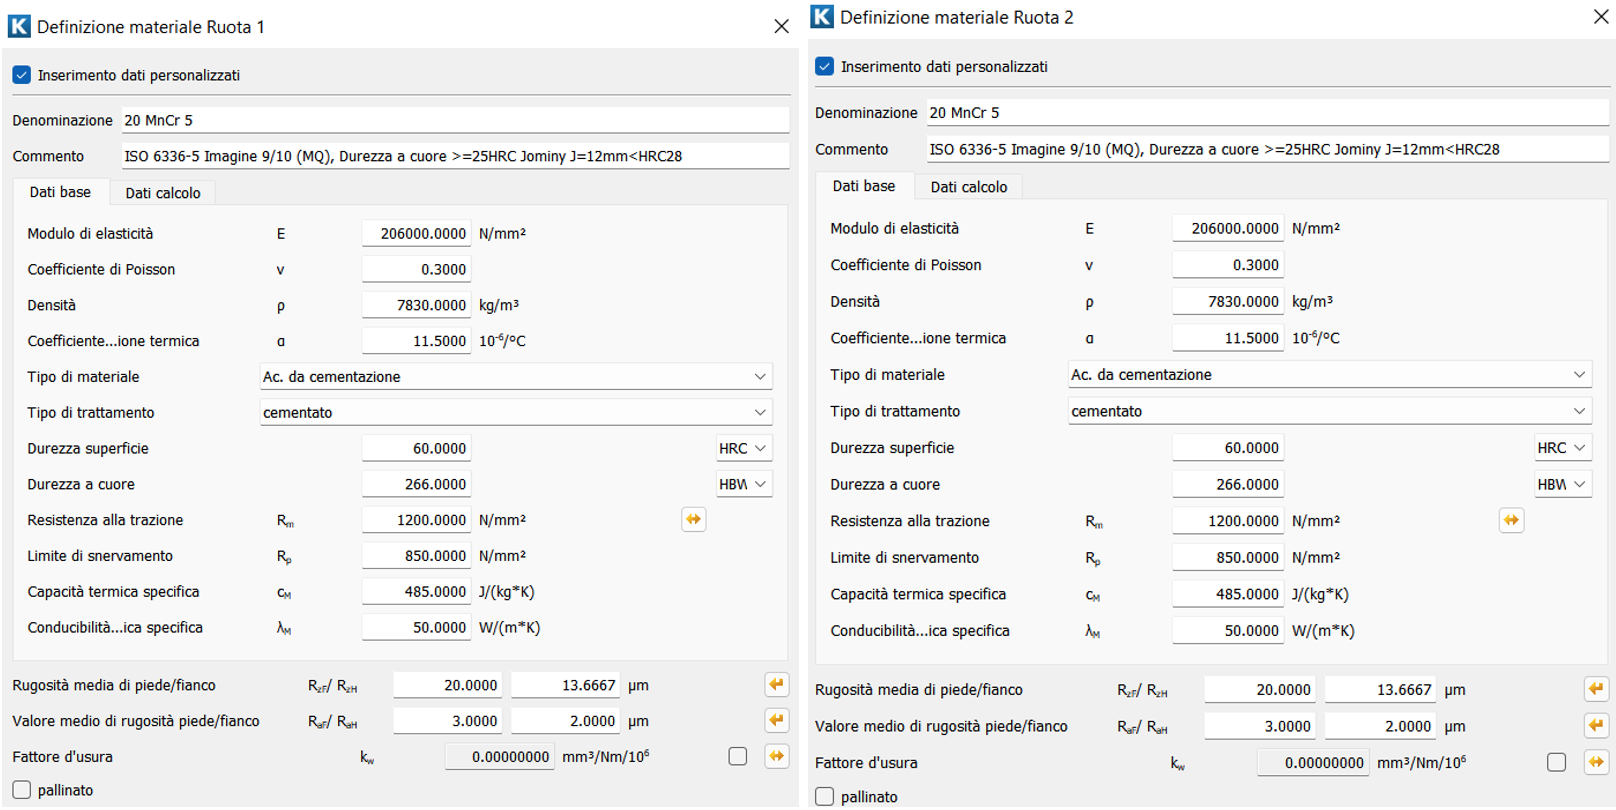
\includegraphics[scale=0.5]{Immagini/RuoteCoppia01.png}
    \caption{Parametri delle ruote della coppia 0 1}
    \label{fig:RuoteCoppia01}
\end{figure}

Il lubrificante utilizzato è \textit{SPIRAX S3 AX 80W-90}, analogo e con le medesime caratteristiche del lubrificante utilizzato per le coppie cilindriche. 
\newpage
Sezione \emph{Procedimento}
\begin{figure}[h]
    \centering
    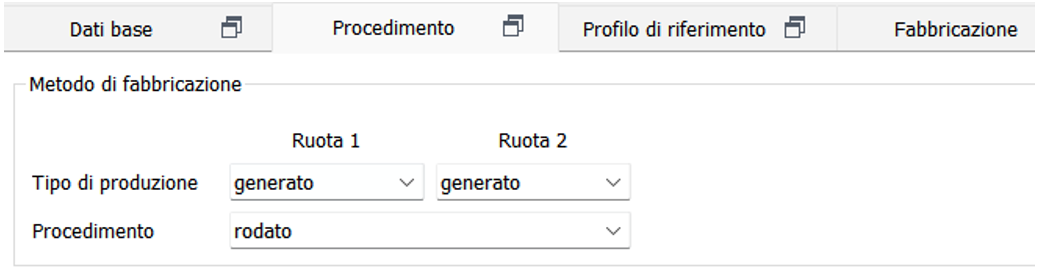
\includegraphics[scale=0.6]{Immagini/ProcedimentoCoppia01.png}
    \caption{Procedimento della coppia 0 1}
    \label{fig:ProcedimentoCoppia01}
\end{figure}

Nel procedimento è necessario inserire il processo di fabbricazione degli ingranaggi, in questo caso rodato.
La tipologia di produzione può essere:
\begin{itemize}
    \item Formato;
    \item Generato (come nella situazione in esame). In generale questa risulta essere la soluzione migliore in quanto fornisce una bombatura al dente, facendo in modo che le pressioni di contatto vengano distribuite lungo una superficie maggiore. 
\end{itemize}

La tipologia di produzione va specificata per entrambe le ruote, e le possibili configurazioni sono:
\begin{itemize}
    \item Pignone generato e corona generata;
    \item Pignone generato e corona formata.
\end{itemize}
Nel primo caso sia pignone che corona presentano una correzione del profilo, mentre nel secondo caso solo il pignone. Quest'ultimo risulta essere vantaggioso per applicazioni in cui si hanno numeri elevati di denti, poiché questo tipo di produzione risulta essere molto più veloce. \\
\\
Sezione \emph{Profilo di riferimento}
\begin{figure}[h]
    \centering
    \includegraphics[scale=0.5]{Immagini/ProfiloRiferimentoCoppia01.png}
    \caption{Profilo di riferimento delle ruote della coppia 0 1}
    \label{fig:ProfiloRiferimentoCoppia01}
\end{figure}

Solitamente per ruote standard si utilizza o prefabbricazione o finitura (senza prefabbricazione), come nel caso in esame. Come profilo di riferimento è buona norma scegliere il Profilo B, in quanto modifica l’altezza del dente andando ad influire sul fattore di ricoprimento. Una volta scelto il profilo di riferimento i dati vengono inseriti in automatico dal Software.
\newpage
Sezione \emph{Fabbricazione}
\begin{figure}[h]
    \centering
    \includegraphics[scale=0.47]{Immagini/FabbricazioneCoppia01.png}
    \caption{Parametri di fabbricazione delle ruote della coppia 0 1}
    \label{fig:FabbricazioneCoppia01}
\end{figure}

Sezione \emph{Tolleranze}
\begin{figure}[h]
    \centering
    \includegraphics[scale=0.47]{Immagini/TolleranzeCoppia01.png}
    \caption{Tolleranze delle ruote della coppia 0 1}
    \label{fig:TolleranzeCoppia01}
\end{figure}

Come tolleranza per lo spessore del dente si è scelto la norma ISO 1328, che come effetto determina uno "smagrimento" del dente.\\
\\
Sezione \emph{Modifiche}
\begin{figure}[h]
    \centering
    \includegraphics[scale=0.47]{Immagini/ModificheCoppia01.png}
    \caption{Modifiche delle ruote della coppia 0 1}
    \label{fig:ModificheCoppia01}
\end{figure}

Le modifiche effettuate sono state:
\begin{itemize}
    \item Ruota 1: bombatura longitudinale, bombatura del profilo centrata sulla lunghezza di rotolamento e correzione angolo d’elica, conica;
    \item Ruota 2: bombatura longitudinale e bombatura del profilo centrata sulla lunghezza di rotolamento. 
\end{itemize}
\newpage
Sezione \emph{Resistenza}
\begin{figure}[h]
    \centering
    \includegraphics[scale=0.47]{Immagini/ResistenzaCoppia01.png}
    \caption{Resistenza delle ruote coppia 0 1}
    \label{fig:ResistenzaCoppia01}
\end{figure}

In questa sezione del software KissSoft vengono inserite Potenza, velocità e momento torcente funzionali al metodo di calcolo ISO10300. La ruota di riferimento da selezionare è chiaramente la ruota motrice e si suppone che il fianco di lavorazione sia il destro. Inoltre, viene inserito manualmente il ciclo di carico fornito dai dati di progetto.\\
\\
Sezione \emph{Fattori}
\begin{figure}[h]
    \centering
    \includegraphics[scale=0.32]{Immagini/FattoriCoppia01.png}
    \caption{Fattori delle ruote della coppia 0 1}
    \label{fig:FattoriCoppia01}
\end{figure}

È necessario definire alcuni fattori, uno su tutti il il fattore di applicazione, che è stato posto unitario siccome si conosce il duty cycle. Se non si conoscesse andrebbe posto maggiore di 1. Inoltre, sia il fattore dinamico che quello trasversale sono posti uguale all’unità.\\
Il fattore di portata $K_{HB}$ è di norma un fattore che deve essere compreso tra 1 e 1,5, a seconda di come sono supportati fisicamente gli ingranaggi: 
\begin{itemize}
    \item $K_{HB}=1$ se nessun asse è montato a sbalzo;
    \item $K_{HB}=1.1$ se un asse è montato a sbalzo;
    \item $K_{HB}=1.25$ se entrambi gli assi sono montati a sbalzo. 
\end{itemize}
Il fattore di flessione alternata $Y_M$ è stato supposto 1, siccome si ha a che fare con un ciclo all’origine. Se si avesse avuto un ciclo alterno allora $Y_M$ sarebbe stato supposto pari a 0.7.
\newpage
Sezione \emph{Analisi del contatto}
\begin{figure}[h]
    \centering
    \includegraphics[scale=0.45]{Immagini/AnalisiContattoCoppia01.png}
    \caption{Analisi del contatto tra le ruote della coppia 0 1}
    \label{fig:AnalisiContattoCoppia01}
\end{figure}

Andando poi in "Grafica" è possibile vedere la Stress Distribution on Tooth 2D. \\
Se la situazione mostra una concentrazione delle tensioni molto accentuata a piede del dente è possibile andare a ri-modificare i fattori di "Modifiche" delle ruote.\\
\\
Ciò che è stato ottenuto in questa analisi è mostrato in Fig.\ref{fig:StressDistributionCoppia01}.
\begin{figure}[h]
    \centering
    \includegraphics[scale=0.6]{Immagini/StressDistributionCoppia01.png}
    \caption{Andamento delle tensioni lungo il fianco del dente}
    \label{fig:StressDistributionCoppia01}
\end{figure}

La sollecitazione è concentrata sulla parte centrale del dente, soluzione ottimale per l’applicazione studiata.\\
\\
Nella sezione "Risultati" è possibile visualizzare tutti i dati ottenuti dall’analisi (in particolare il fattore di ricoprimento e i valori dei coefficienti di sicurezza).\\
\\
La verifica a resistenza risulta soddisfatta per i seguenti valori:
\begin{itemize}
    \item Sicurezza al piede del dente (Bending), $S_F>1.3$;
    \item Sicurezza al finaco del dente (Pitting), $S_H>1.1$.
\end{itemize}
\newpage
\begin{figure}[h]
    \centering
    \includegraphics[scale=0.45]{Immagini/RisultatiCoppia01.png}
    \caption{Risultati dell'analisi del contatto tra le ruote della coppia 0 1}
    \label{fig:RisultatiCoppia01}
\end{figure}

Il Software fornisce anche una rappresentazione 3D di massima dell’accoppiamento
\begin{figure}[h]
    \centering
    \includegraphics[scale=0.5]{Immagini/GeometriaCoppia01.png}
    \caption{Rappresentazione geometrica 3D della coppia di ruote 0 1}
    \label{fig:GeometriaCoppia01}
\end{figure}

\paragraph{Coppia conica 2 3}Definizione dei dati di base della coppia conica.  
\begin{figure}[h]
    \centering
    \includegraphics[scale=0.45]{Immagini/Coppia23.png}
    \caption{Dati di base coppia 2 3}
    \label{fig:Coppia23}
\end{figure}
\newpage
A seguito di diversi tentativi quindi, per la seconda coppia conica è stato scelto un numero di denti pari a 19 per la ruota 1 e pari a 42 per la ruota 2. Il modulo è stato supposto pari a 4 mm, la larghezza del dente pari a 28 mm, l’angolo di pressione $20^\circ$ e un diametro primitivo della seconda ruota pari a 194 mm, ideale per rispettare gli ingombri disponibili. La qualità degli ingranaggi pari a 9 (DIN3965). Il materiale scelto per entrambe le ruote è un acciaio da cementazione 20MnCr5, con un carico di rottura $R_m$ pari a $1200\ N/mm^2$ e un carico di snervamento $R_s$ pari a 850 $N/mm^2$. 
\begin{figure}[h]
    \centering
    \includegraphics[scale=0.5]{Immagini/RuoteCoppia23.png}
    \caption{Parametri delle ruote della coppia 2 3}
    \label{fig:RuoteCoppia23}
\end{figure}

Il lubrificante utilizzato è \textit{SPIRAX S3 AX 80W-90}, analogo e con le medesime caratteristiche del lubrificante utilizzato per le coppie cilindriche. \\
\\
Sezione \emph{Procedimento}
\begin{figure}[h]
    \centering
    \includegraphics[scale=0.6]{Immagini/ProcedimentoCoppia23.png}
    \caption{Procedimento della coppia 2 3}
    \label{fig:ProcedimentoCoppia23}
\end{figure}

La tipologia di produzione può essere:
\begin{itemize}
    \item Formato;
    \item Generato (come nella situazione in esame). In generale questa risulta essere la soluzione migliore in quanto fornisce una bombatura al dente, facendo in modo che le pressioni di contatto vengano distribuite lungo una superficie maggiore. 
\end{itemize}

La tipologia di produzione va specificata per entrambe le ruote, e le possibili configurazioni sono:
\begin{itemize}
    \item Pignone generato e corona generata;
    \item Pignone generato e corona formata.
\end{itemize}
Nel primo caso sia pignone che corona presentano una correzione del profilo, mentre nel secondo caso solo il pignone. Quest'ultimo risulta essere vantaggioso per applicazioni in cui si hanno numeri elevati di denti, poiché questo tipo di produzione risulta essere molto più veloce. \\
\\
Sezione \emph{Profilo di riferimento}
\begin{figure}[h]
    \centering
    \includegraphics[scale=0.45]{Immagini/ProfiloRiferimentoCoppia23.png}
    \caption{Profilo di riferimento delle ruote della coppia 2 3}
    \label{fig:ProfiloRiferimentoCoppia23}
\end{figure}

Solitamente per ruote standard si utilizza o prefabbricazione o finitura (senza prefabbricazione), come nel caso in esame. Come profilo di riferimento è buona norma scegliere il Profilo B, in quanto modifica l’altezza del dente andando ad influire sul fattore di ricoprimento. Una volta scelto il profilo di riferimento i dati vengono inseriti in automatico dal Software.\\
\\
Sezione \emph{Fabbricazione}
\begin{figure}[h]
    \centering
    \includegraphics[scale=0.47]{Immagini/FabbricazioneCoppia23.png}
    \caption{Parametri di fabbricazione delle ruote della coppia 2 3}
    \label{fig:FabbricazioneCoppia23}
\end{figure}
\newpage
Sezione \emph{Tolleranze}
\begin{figure}[h]
    \centering
    \includegraphics[scale=0.47]{Immagini/TolleranzeCoppia23.png}
    \caption{Tolleranze delle ruote della coppia 2 3}
    \label{fig:TolleranzeCoppia23}
\end{figure}

Come tolleranza per lo spessore del dente si è scelto la norma ISO 1328, che come effetto determina uno "smagrimento" del dente.\\
\\
Sezione \emph{Modifiche}
\begin{figure}[h]
    \centering
    \includegraphics[scale=0.47]{Immagini/ModificheCoppia23.png}
    \caption{Modifiche delle ruote della coppia 2 3}
    \label{fig:ModificheCoppia23}
\end{figure}

Le modifiche effettuate sono state:
\begin{itemize}
    \item Ruota 1: bombatura longitudinale e del profilo, centrata sulla lunghezza di rotolamento;
    \item Ruota 2: bombatura longitudinale, bombatura del profilo centrata sulla lunghezza di rotolamento e correzione angolo d'elica conica. 
\end{itemize}
\newpage
Sezione \emph{Resistenza}
\begin{figure}[h]
    \centering
    \includegraphics[scale=0.47]{Immagini/ResistenzaCoppia23.png}
    \caption{Resistenza delle ruote coppia 2 3}
    \label{fig:ResistenzaCoppia23}
\end{figure}

In questa sezione del software KissSoft vengono inserite potenza, velocità e momento torcente funzionali al metodo di calcolo ISO10300. La ruota di riferimento da selezionare è chiaramente la ruota motrice e si suppone che il fianco di lavorazione sia il destro. Inoltre, viene inserito manualmente il ciclo di carico fornito dai dati di progetto.\\
\\
Sezione \emph{Fattori}
\begin{figure}[h]
    \centering
    \includegraphics[scale=0.45]{Immagini/FattoriCoppia23.png}
    \caption{Fattori delle ruote della coppia 2 3}
    \label{fig:FattoriCoppia01}
\end{figure}

È necessario definire alcuni fattori, uno su tutti il il fattore di applicazione, che è stato posto unitario siccome si conosce il duty cycle. Se non si conoscesse andrebbe posto maggiore di 1. Inoltre, sia il fattore dinamico che quello trasversale sono posti uguale all’unità.\\
Il fattore di portata $K_{HB}$ è di norma un fattore che deve essere compreso tra 1 e 1,5, a seconda di come sono supportati fisicamente gli ingranaggi: 
\begin{itemize}
    \item $K_{HB}=1$ se nessun asse è montato a sbalzo;
    \item $K_{HB}=1.1$ se un asse è montato a sbalzo;
    \item $K_{HB}=1.25$ se entrambi gli assi sono montati a sbalzo. 
\end{itemize}
Il fattore di flessione alternata $Y_M$ è stato supposto 1, siccome si ha a che fare con un ciclo all’origine. Se si avesse avuto un ciclo alterno allora $Y_M$ sarebbe stato supposto pari a 0.7.
\newpage
Sezione \emph{Analisi del contatto}
\begin{figure}[h]
    \centering
    \includegraphics[scale=0.45]{Immagini/AnalisiContattoCoppia23.png}
    \caption{Analisi del contatto tra le ruote della coppia 2 3}
    \label{fig:AnalisiContattoCoppia23}
\end{figure}

Andando poi in "Grafica" è possibile vedere la Stress Distribution on Tooth 2D. \\
Se la situazione mostra una concentrazione delle tensioni molto accentuata a piede del dente è possibile andare a ri-modificare i fattori di "Modifiche" delle ruote.\\
\\
Ciò che è stato ottenuto in questa analisi è mostrato in Fig.\ref{fig:StressDistributionCoppia23}.
\begin{figure}[h]
    \centering
    \includegraphics[scale=0.6]{Immagini/StressDistributionCoppia23.png}
    \caption{Andamento delle tensioni lungo il fianco del dente}
    \label{fig:StressDistributionCoppia23}
\end{figure}

La sollecitazione è concentrata sulla parte centrale del dente, soluzione ottimale per l’applicazione studiata.\\
\newpage
Nella sezione "Risultati" è possibile visualizzare tutti i dati ottenuti dall’analisi (in particolare il fattore di ricoprimento e i valori dei coefficienti di sicurezza). \\
La verifica a resistenza risulta soddisfatta per i seguenti valori:
\begin{itemize}
    \item Sicurezza al piede del dente (Bending), $S_F>1.3$;
    \item Sicurezza al finaco del dente (Pitting), $S_H>1.1$.
\end{itemize}
\begin{figure}[h]
    \centering
    \includegraphics[scale=0.49]{Immagini/RisultatiCoppia23.png}
    \caption{Risultati dell'analisi del contatto tra le ruote della coppia 2 3}
    \label{fig:RisultatiCoppia23}
\end{figure}

Il Software fornisce anche una rappresentazione 3D di massima dell’accoppiamento
\begin{figure}[h]
    \centering
    \includegraphics[scale=0.55]{Immagini/GeometriaCoppia23.png}
    \caption{Rappresentazione geometrica 3D della coppia di ruote 2 3}
    \label{fig:GeometriaCoppia23}
\end{figure}































